\documentclass{article}
\usepackage[utf8]{inputenc}
\usepackage{amsmath}
\usepackage{amssymb}
\usepackage{authblk}
\usepackage{longtable}
\usepackage{lscape}
\usepackage{graphicx}
\usepackage{lipsum}
\usepackage{wrapfig}
\usepackage{smartdiagram}
\usepackage{subcaption}
\graphicspath{ {./plots/} }
\DeclareGraphicsExtensions{.png,.pdf}

\title{Lallemand Yeast Strain 7442 Mutation Analysis}
\author{Peeter Meos, Liubov Kaes, Tanel Peet, Ott Keki{\v s}ev}
%\texttt{peeter.meos@proekspert.ee}
\affil{Proekspert AS}
%\and
%\texttt{liubov.kyaes@proekspert.ee} 
%\and
%\texttt{tanel.peet@proekspert.ee}
%\and
%\texttt{ott.kekisev@proekspert.ee}
%}

\date{May 2019}

\begin{document}
\maketitle

\tableofcontents
\listoffigures

\section{Introduction}
The purpose of this study is to investigate and provide possible insight into the causes of undesirable mutations in yeast strain 7442. Lallemand has established a hypothesis, that the mutations could be caused by an unknown and unfavorable combination of parameters of the production processes. Since the parameter data  of the processes are measured and collected automatically, it should be possible to test that hypothesis using quantitative methods.

Therefore, this analysis, while limited in scope, takes a first look at the collected data. The study looks at the quality and usability of the data, performs feature reduction and takes first steps in modelling and predicting the mutation. Additionally, in the end we provide recommendations how to make the data collection, processing and analysis more automated, holistic and less error prone as opposed to current partly manual data collection.

\section{Process Description}
Process of yeast fermentation, as described by Lallemand, consists of steps F1-F8. The study is taking a look at steps F2 (seed culture feedbatch) and steps F4 and F5 (semicultural feedbatch and or commercial batches). Even though the data for other batches (ie strains) are present, the labelling is not. Therefore there is not enough information on other batches to perform the study.

\begin{figure}[ht]
    \centering
    \smartdiagramset{
        uniform color list=gray!150!black for 4 items
        }
    \smartdiagram[sequence diagram]{F1, F2,F4,F5-8}
    \caption{Sequence of fermentation steps}
    \label{fig:process_steps}
\end{figure}


\section{Data Preparation}
The time series data describing the process arrived in a form of CSV files. The automation system providing the data had split the data vertically into a number of separate files. That is the variables describing the data are grouped into separate files, with one file consisting the entire length of time series (March - December 2018). The process steps were as follows: F2, F4, F5, F6, F7, F8. Additionally we were given data on three processes: CSep, MO and SP. The automation system collects the data at 10 minute interval, but in the time stamps themselves between the respective CSV files vary within that interval (in simpler terms, the timestamps on lines don't match). That is, even though all CSV files for a given process step have the same number of rows, the time stamps for these rows are shifted but remain inside 10 minute window. Therefore we rounded all time stamps to the nearest smaller 10 minute point. That allowed the time stamps to match and data to be merged.

\subsection{Batch Identification}
The F-process data were time stamped and also enriched with process time field. Therefore it was easy for these process steps to mark the batches. When the field \texttt{step\_time} was zero, the production line was considered idle. The value change from zero to non-zero was considered as a marker for start of production batch. Counting cumulatively the number of start markers allowed us to give a sequence number for each production batch in each F-production step. Table \ref{tab:new_attributes} summarizes the new variables created.

\begin{table}[ht]
    \centering
    \begin{tabular}{l p{9.5cm}}
        Variable &  Description \\
        \hline
        dtg & periodic time stamp (period in 10 minutes) \\
        active &   	    active =0   Production Line stopped \newline
                        active =1   Production Line running
        \\
        start&	        batch start indicator \newline
                        start=1 new batch begins (started) \newline
                        start=0 no change in cycle
        \\
        cycle&	batch sequence number \newline
                cycle = 0 no batch running \newline
                cycle=$1\ldots N$  active batch number (serial number)
        \\
        \hline
    \end{tabular}
    \caption{Description of new variables}
    \label{tab:new_attributes}
\end{table}

\subsection{Labelling}
As extra data we were given labels for 12 production batches. The labels were titled ''reject'', ''restrict'' and ''release''. In order to know which batches to label were additionally given production records in a form of PDF files with handwritten notes. A production record contained dates for process steps of F2 and following F4 or F5. We matched manually those dates with our labelling described above. We assumed that the dates in the PDF files marked the \emph{beginning} of the production step. However, in two cases of F2 we were not able to establish that match and picked the \emph{preceding} batch label in the data. The rationale for that the date was recorded during the batch and the production itself had started the previous day. This proved again, that manual data recording is inherently inconsistent and error prone. Therefore, one of our recommendations of our short analysis is to preferably automate the process. If the full automation is not possible, the HMI\footnote{HMI - Human Machine Interface} should be developed that ensures the consistency of times tamps in the recorded data. The full set of recommendations are described in more detail in the last section of this report. The batch numbers in the data with the respective labels are displayed in the table \ref{tab:batches} below.

\begin{table}[ht]
    \centering
    \begin{tabular}{l p{1cm} p{1cm} p{1cm} l l}
        & \multicolumn{3}{ c }{Batch production dates} \\
        \hline
         Batch & F2 &  F4 &  F5 &  & Comment \\
        \hline
        4109&4/17    & 4/19    &         & reject& \\
        4141&5/18    & 5/21    &         & reject& \\
        4147&5/25    & 5/27    &         & release&Data issue\\
        4151&5/29    & 6/1     &         & release&\\
        4165&6/12    & 6/14    &         & release&\\
        4201&7/18    & 7/20    &         & release&\\
        4242&8/28    & 8/30    &         & reject&Data issue\\
        4266&9/21    & 9/23    &         & restrict&Data issue\\
        4308&11/2    & 11/4    &         & release&\\
        4320&11/14   & 11/16   &         & restrict&\\
        5283&10/8    &         & 10/10   & release&\\
        5292&10/17   &         & 10/19   & reject&\\
        \hline
    \end{tabular}
    \caption{Labelled production batches}
    \label{tab:batches}
\end{table}


\section{Exploratory Data Analysis}
Initially for EDA we concentrated to process steps F2 and F4 since majority of the labelled data resided within those two steps. After completing those we also took a look at F5 and the remaining data sets. The data itself is of acceptable quality with no additional changes necessary. The time series inside a given process step contained, however, various levels of information. Some series were almost exclusively either zero, static, or missing. Since these series do not have at least within this study any explanatory power, we cut these series out. The table below displays the time series that were left to describe each process. The processes displayed on Figures \ref{fig:f2series}, \ref{fig:f4series} and \ref{fig:f5series}.

\begin{figure}[ht]
    \centering
    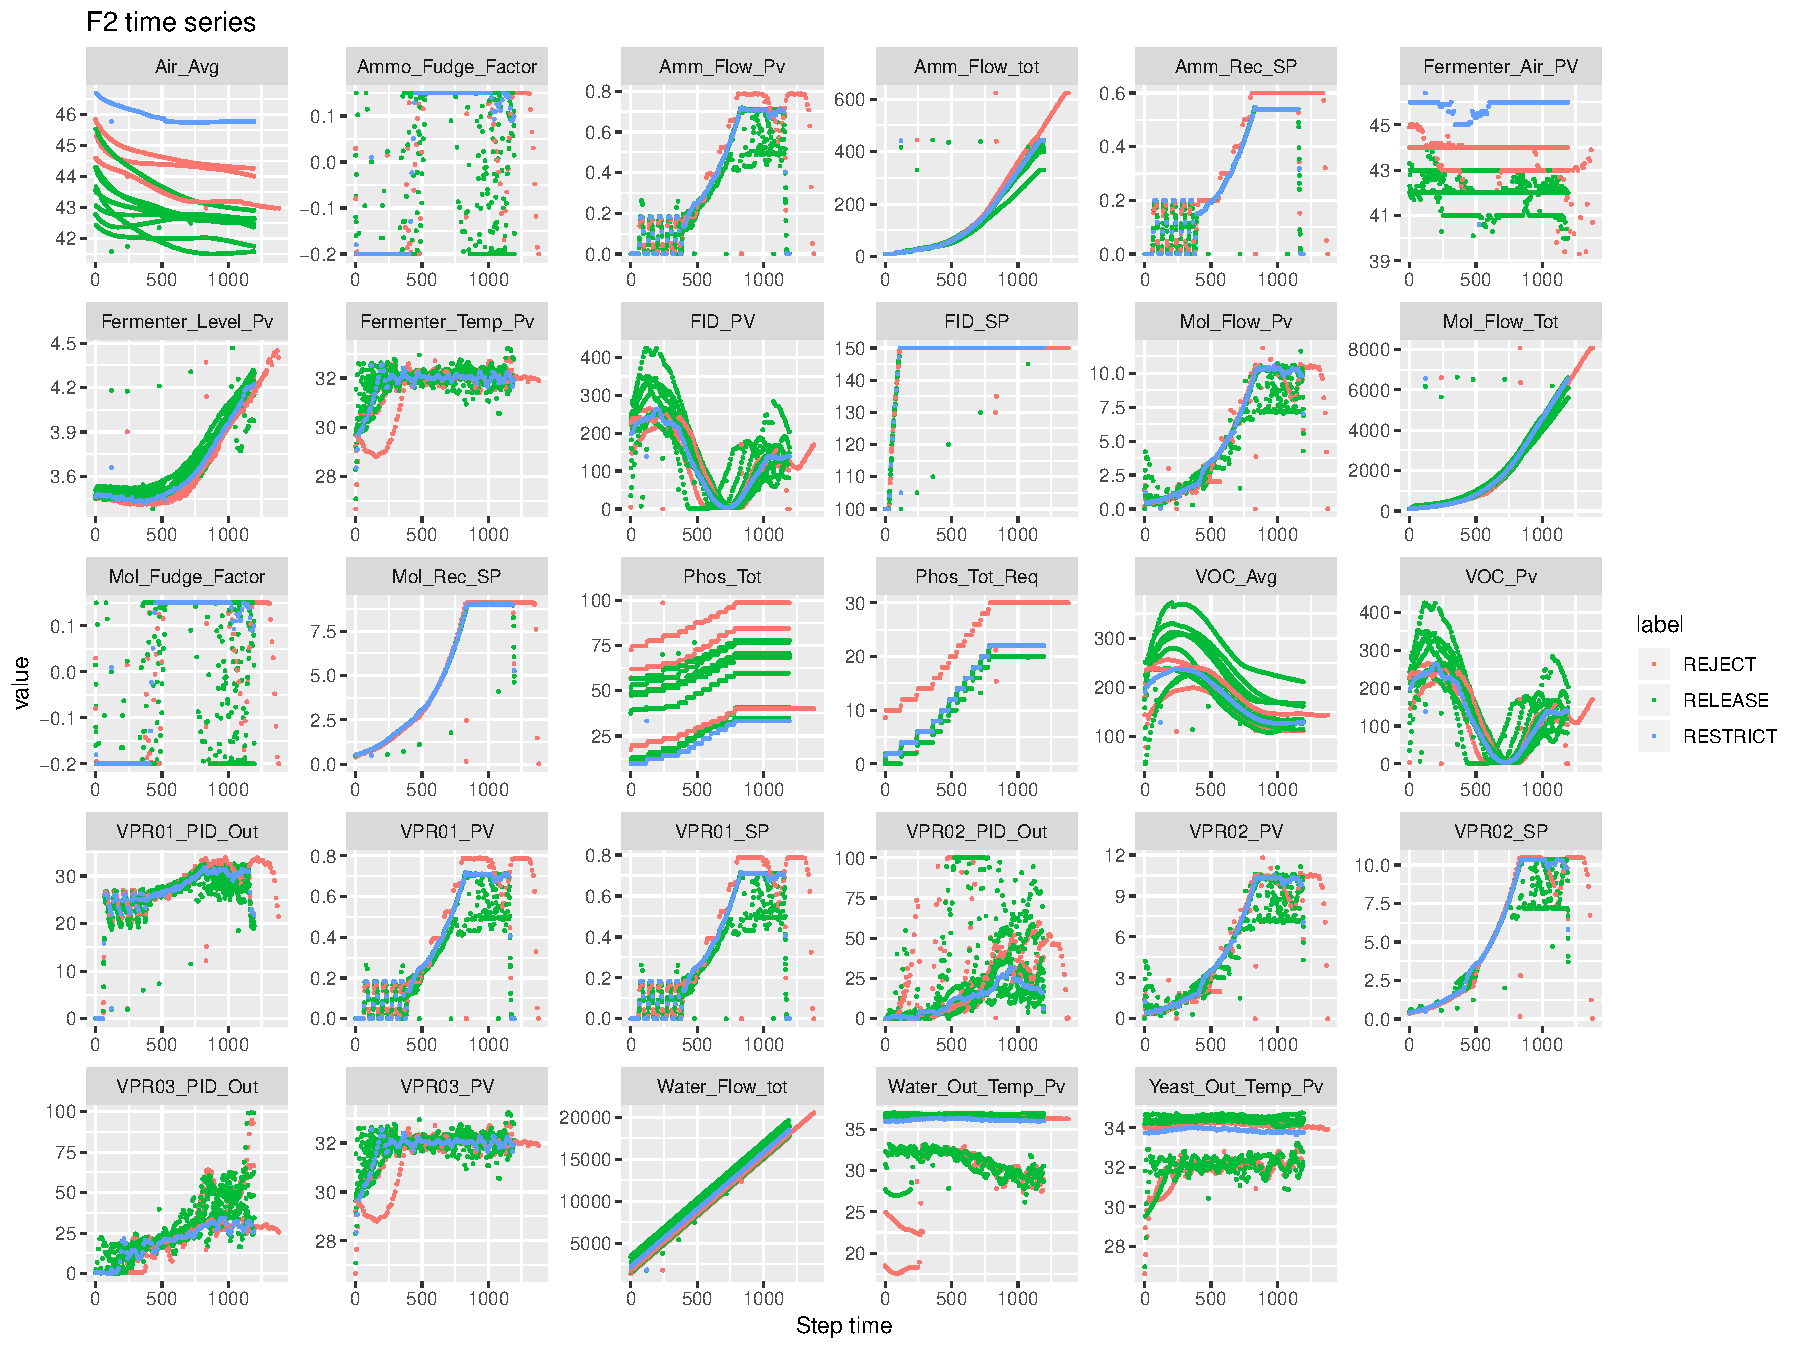
\includegraphics[width=1.0\textwidth]{f2_plot}
    \caption{Overview of labelled F2 production batches}
    \label{fig:f2series}
\end{figure}

\begin{figure}[ht]
    \centering
    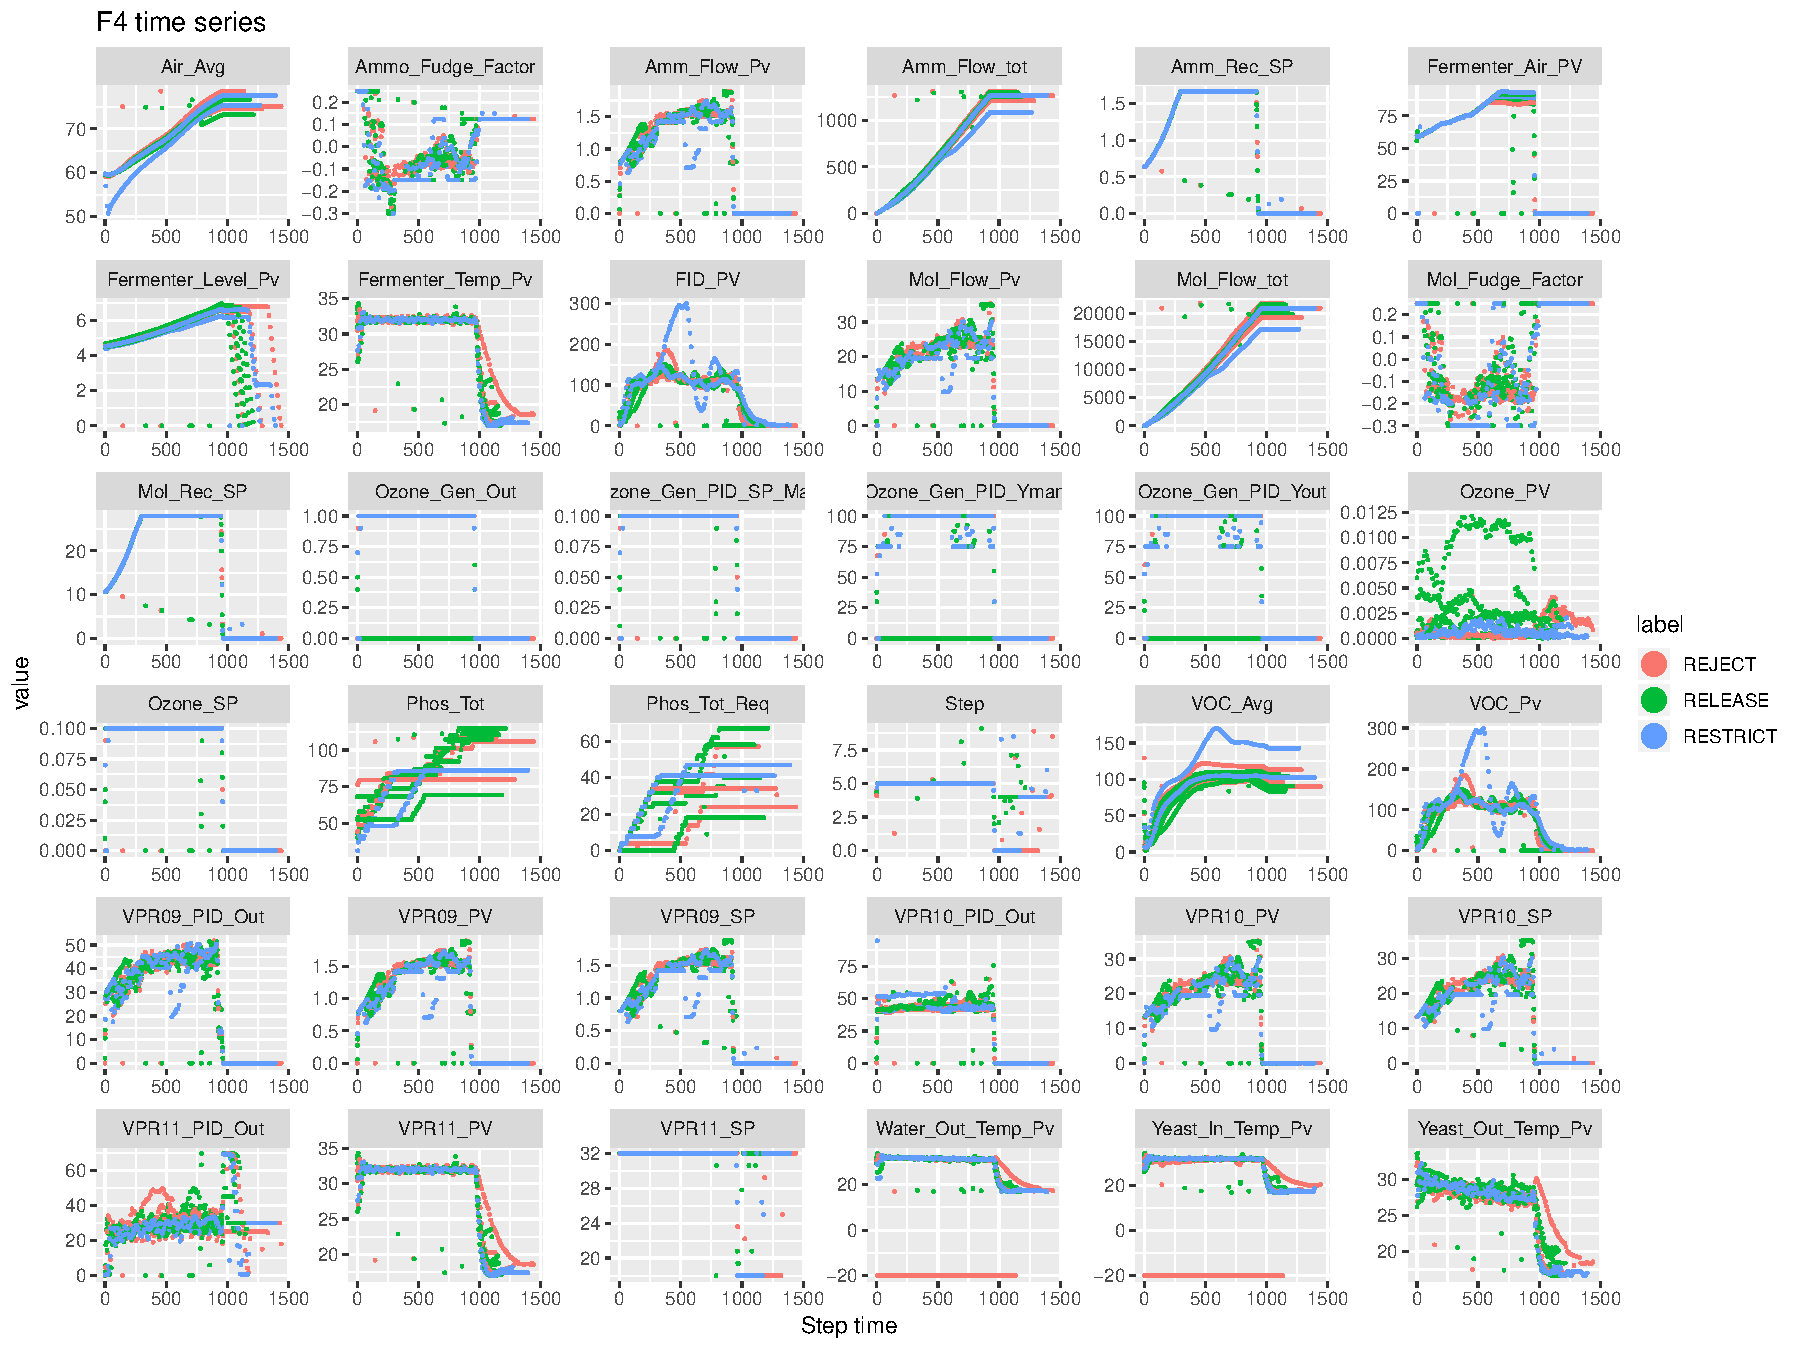
\includegraphics[width=1.0\textwidth]{f4_plot}
    \caption{Overview of labelled F4 production batches}
    \label{fig:f4series}
\end{figure}


\begin{figure}[ht]
    \centering
    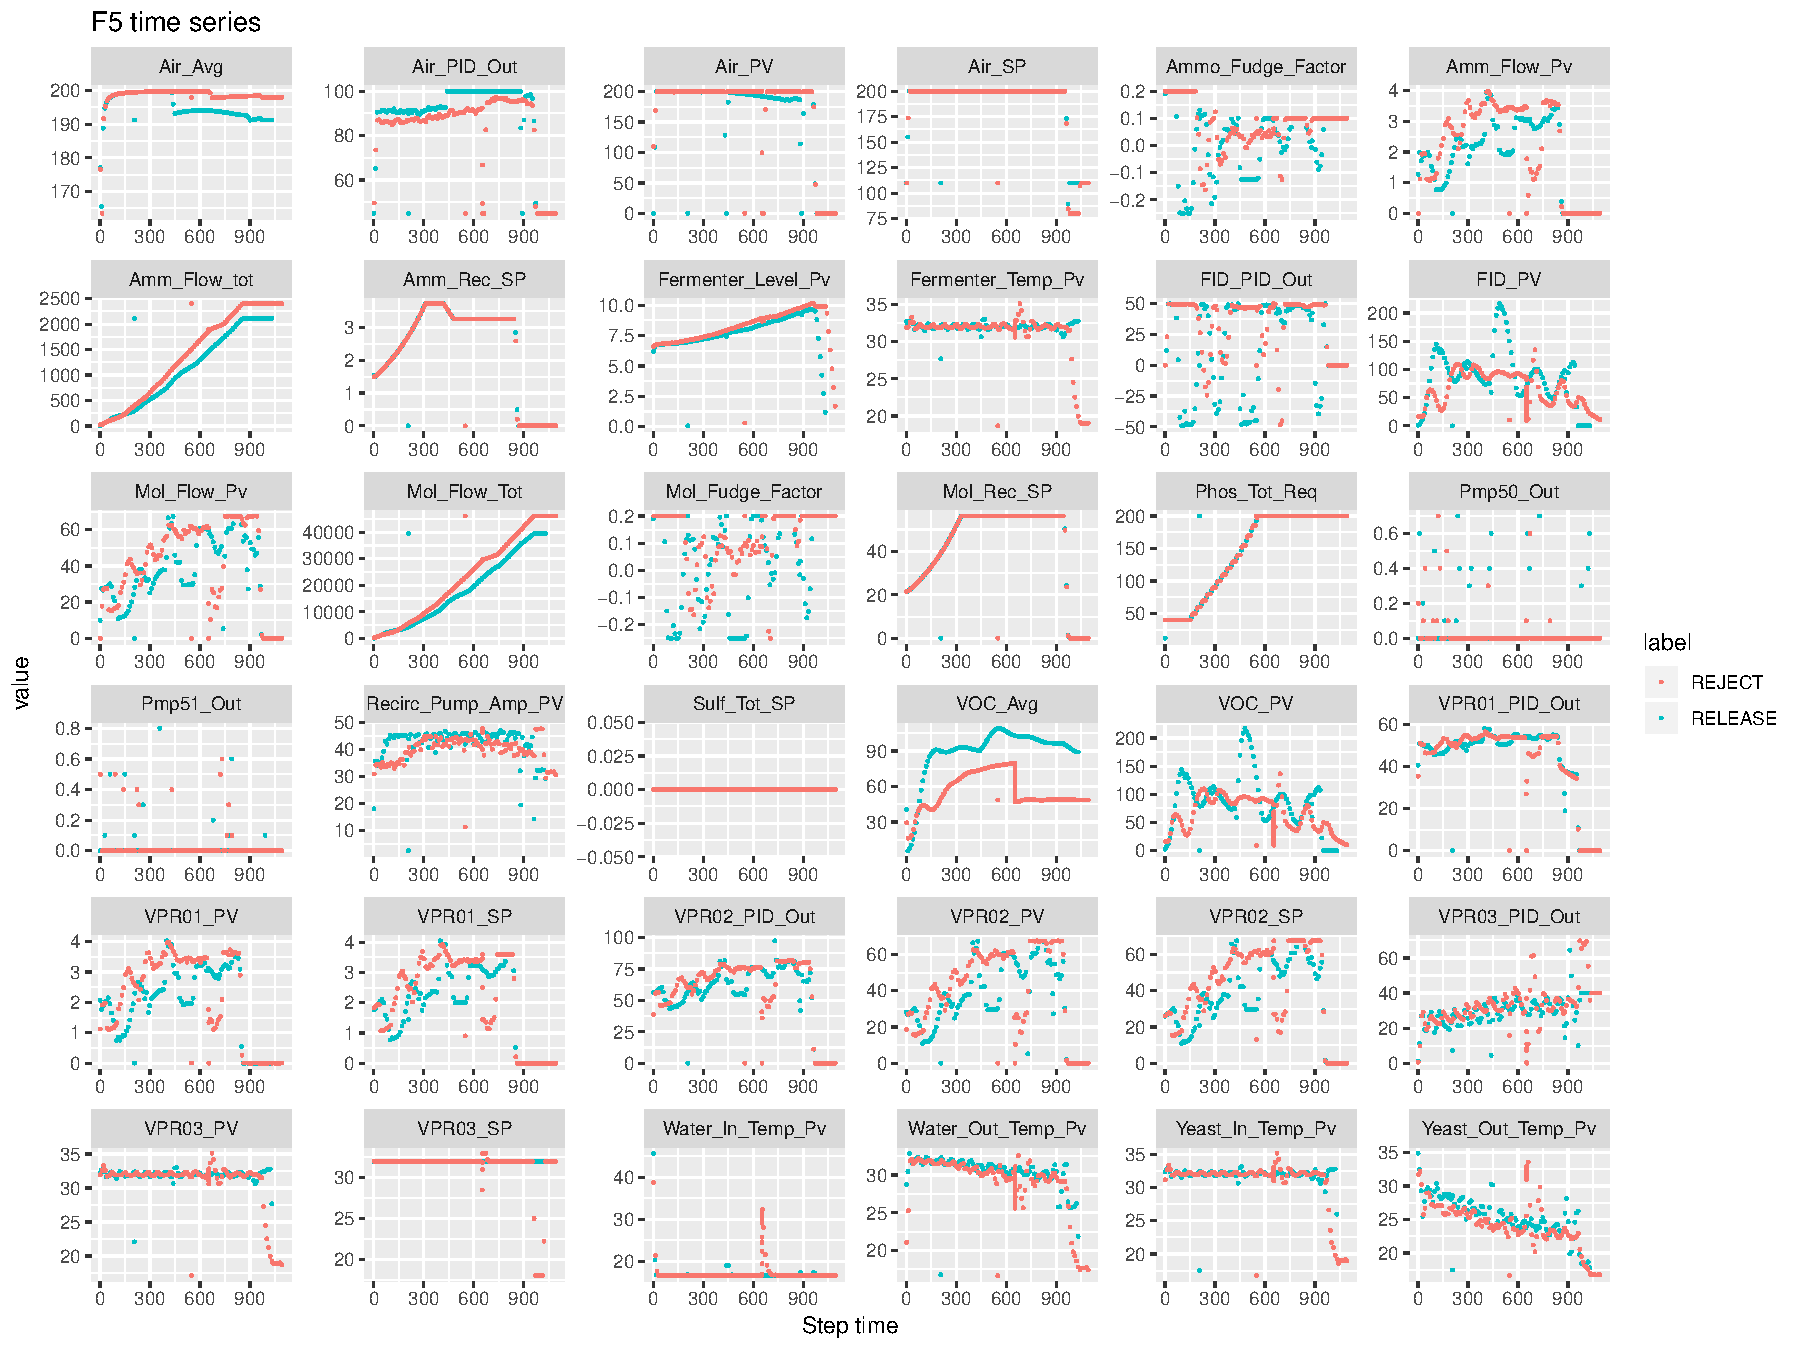
\includegraphics[width=1.0\textwidth]{f5_plot}
    \caption{Overview of labelled F5 production batches}
    \label{fig:f5series}
\end{figure}

\section{Feature Engineering}
Analysis of variables based on step times to identify some interruption in data recordings or process.  (parameters collection and representation based on step time and time stamps).

According to provided quality control results (seed and status) information it was possible to explore F2, F4 and F5 yeast fermentation process data. The new labelled dataset was created containing the observations with \emph{manually identified batches and related statuses} (label whether was it rejected, released or restricted release).

\subsection{Study of variables}
Using multivariate Principal Component Analysis (PCA) method for reducing dimensionality. The method determines the number of principal components and help to identify outliers. The original data set had a plenty correlated and uncorrelated variables and dimensionality reduction can be a very useful step for visualizing and processing high-dimensional data sets.  PCA was used for data understanding as it allowing most of the variability to be explained using fewer variables.

The essence of PCA is to map data points that lie in a high dimensional space into lower dimensional space without significant loss of information. When data has strongly correlated features, then calculating the eigenvectors and eigenvalues of the covariance matrix provides a new lower dimensional orthogonal basis for the data. Picking out a basis from those eigenvectors (for instance 4-5 vectors with most explanatory power) allows us to reduce dimensionality in our case from approximately $\mathbb{R}^{20} \to \mathbb{R}^4$. The downside of this, however, is the interpretability. The actual real life meaning of new transformed axes may not be intuitive and explainable by real world processes. Therefore, PCA should always be complimented by actual domain knowledge of the processes.

PCA was performed in the following steps: first determining the number of desired principal components, then interpreting each principal component in terms of the original variables and and lastly identifying the outliers. Therefore, the first step of exploratory analysis was performing preliminary feature selection operations in order to bring the number of variables to a manageable range.
 
 \subsection{Classification}
F2, F4, F5 Data Classification.  For prediction a status the Linear Discriminant Analysis (LDA) was applied on data transformed by PCA afterwards. The expectation was, that performing PCA before LDA modelling should give a little better results. LDA explicitly attempts to model the difference between the classes of data and is used when groups are known \emph{a priori}.  LDA was applied on labelled samples and then to unlabeled F2, F4 and F5 data.
 
Analysis of variables to find out deviations from mean values between status groups. Box plotting.  Applied on classified data set (predicted labels/statuses) 

\subsection{Tools}
Since the dataset was rather limited in size, no complex mechanisms for data storage and processing, such as parallel processing, big data storage, or even regular SQL data bases were needed. 

All required data analysis and inference was done in R. PCA was performed using the built-in R functions \texttt{prcomp()}, \texttt{princomp()}. For visualization the study used R packages \texttt{factoextra} and \texttt{ggplot2} with its respective extensions such as facetting. R package MASS was used for LDA. 

% Analysis section
\section{Analysis}
\label{sec:analysis}
\subsection{Analysis of F2}
For analysis the F2 process step contained the significantly more data compared to F4 and F5 which makes the results somewhat more reliable. However, since the sample size is nevertheless small, the results need to be taken as inconclusive and in need of additional research and interpretation by someone with deep knowledge of the process. It should be noted, that the classification into rejected, released and restricted release categories is not balanced with most of the data residing in release category. This is naturally reflected in the distribution of the data as depicted in Figure \ref{fig:f2_sample}. This figure does not include time series that are either static or otherwise lack significant information. 

It is immediately evident, that in most time series, the batches that were later classified as ``rejected'' contain significantly more variance than the other two categories. This cannot be explained by just other categories having different quantities of data.

\begin{figure}[ht!]
    \centering
    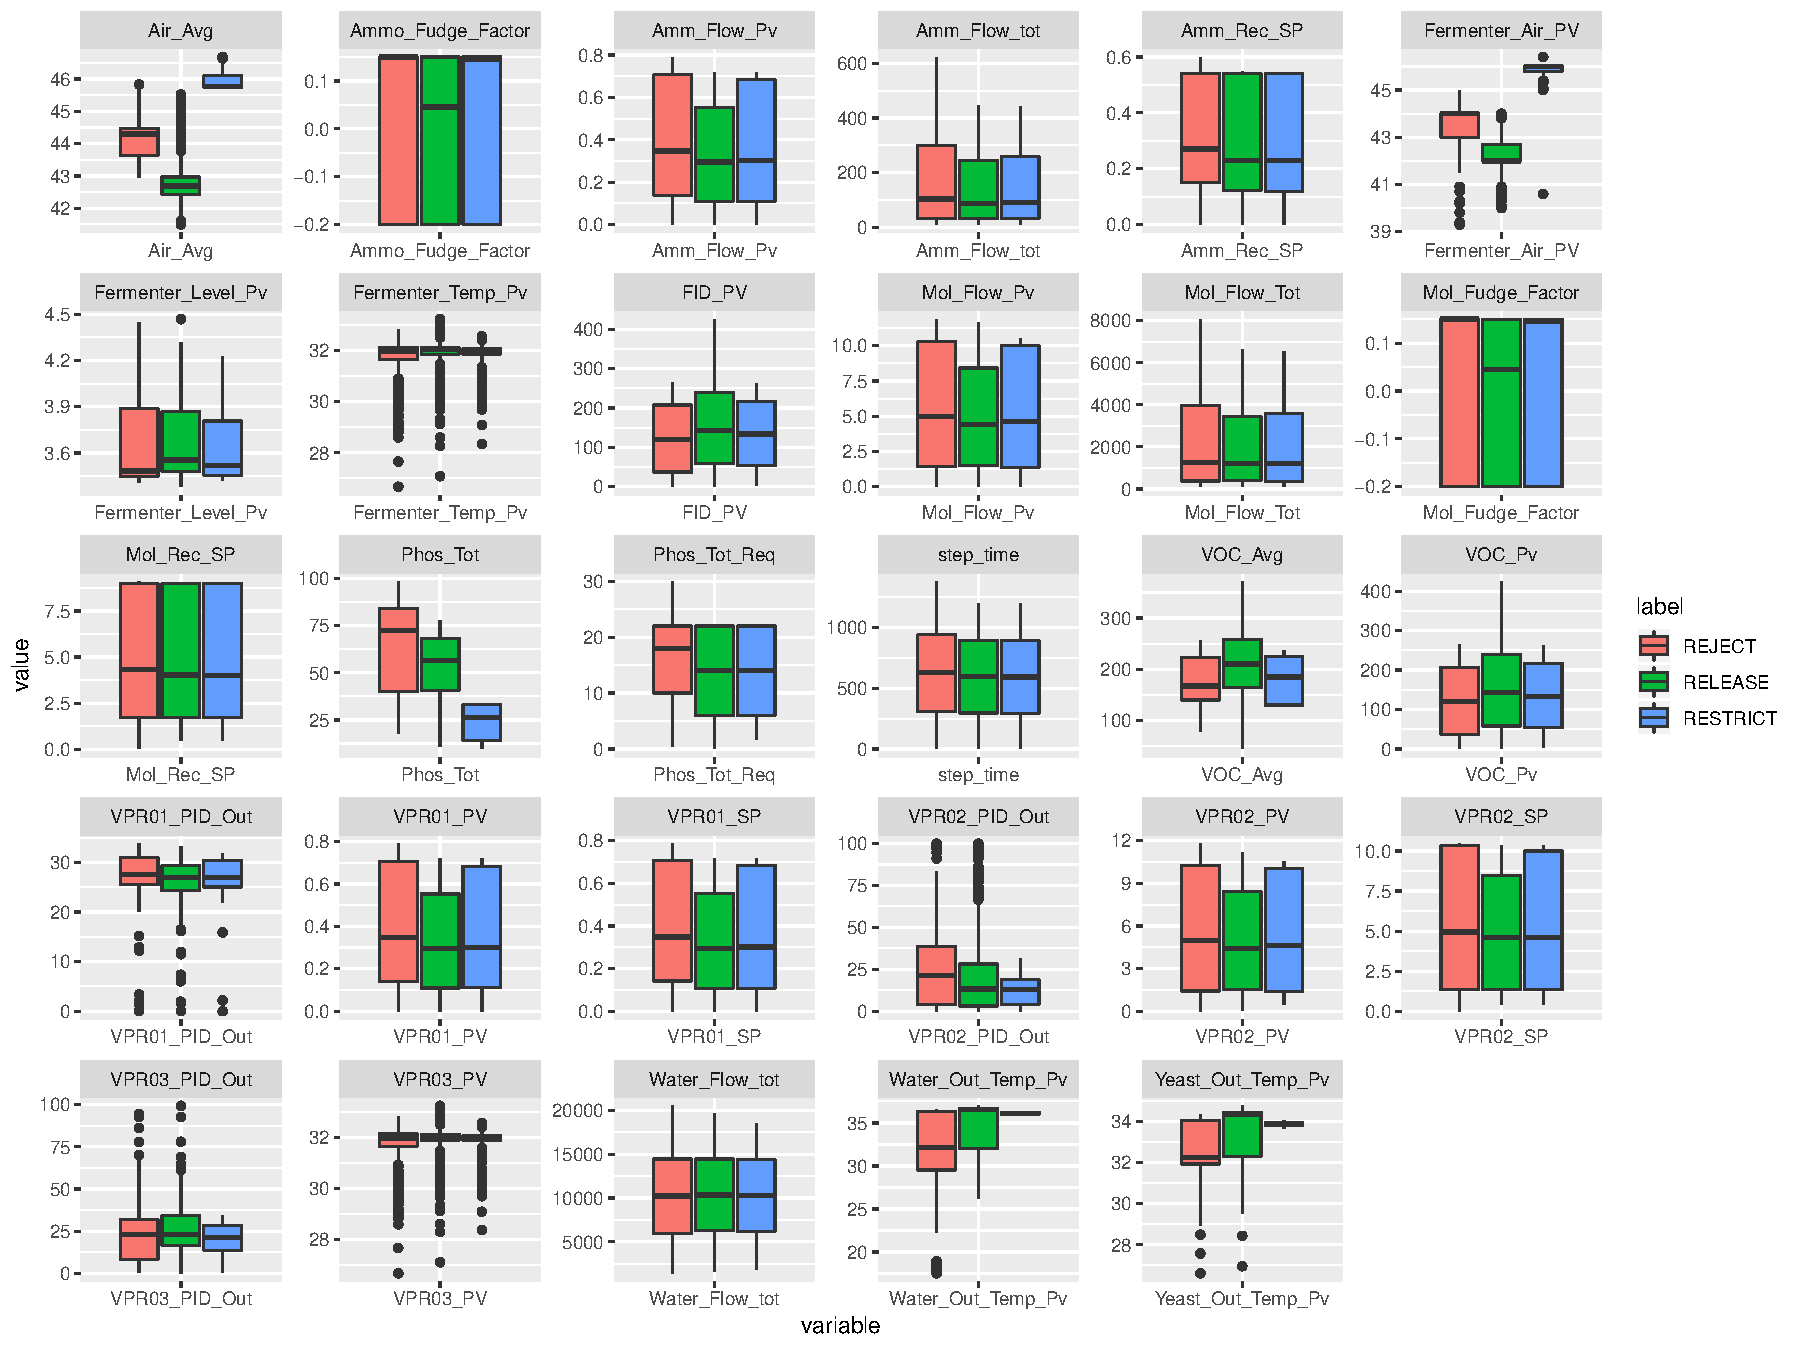
\includegraphics[width=1.0\textwidth]{plots/f2-sample.pdf}
    \caption{F2 sample}
    \label{fig:f2_sample}
\end{figure}

This pattern continued after normalizing the variables to a common scale and performing PCA feature reduction and LDA clustering. As can be seen from Figure \ref{fig:f2_predicted}, also the predicted labels of the production batches follow the same trend of ``rejected'' having significantly larger amount of variance. Since as of this writing, the authors lack profound knowledge about the process, it is difficult to say, if the claim, that variance in F2 process parameters is the cause of undesired mutations, has any substance. However, we believe, that there is enough evidence to do additional research on the effects of F2 process stability on the quality of the yeast.

\begin{figure}[ht!]
    \centering
    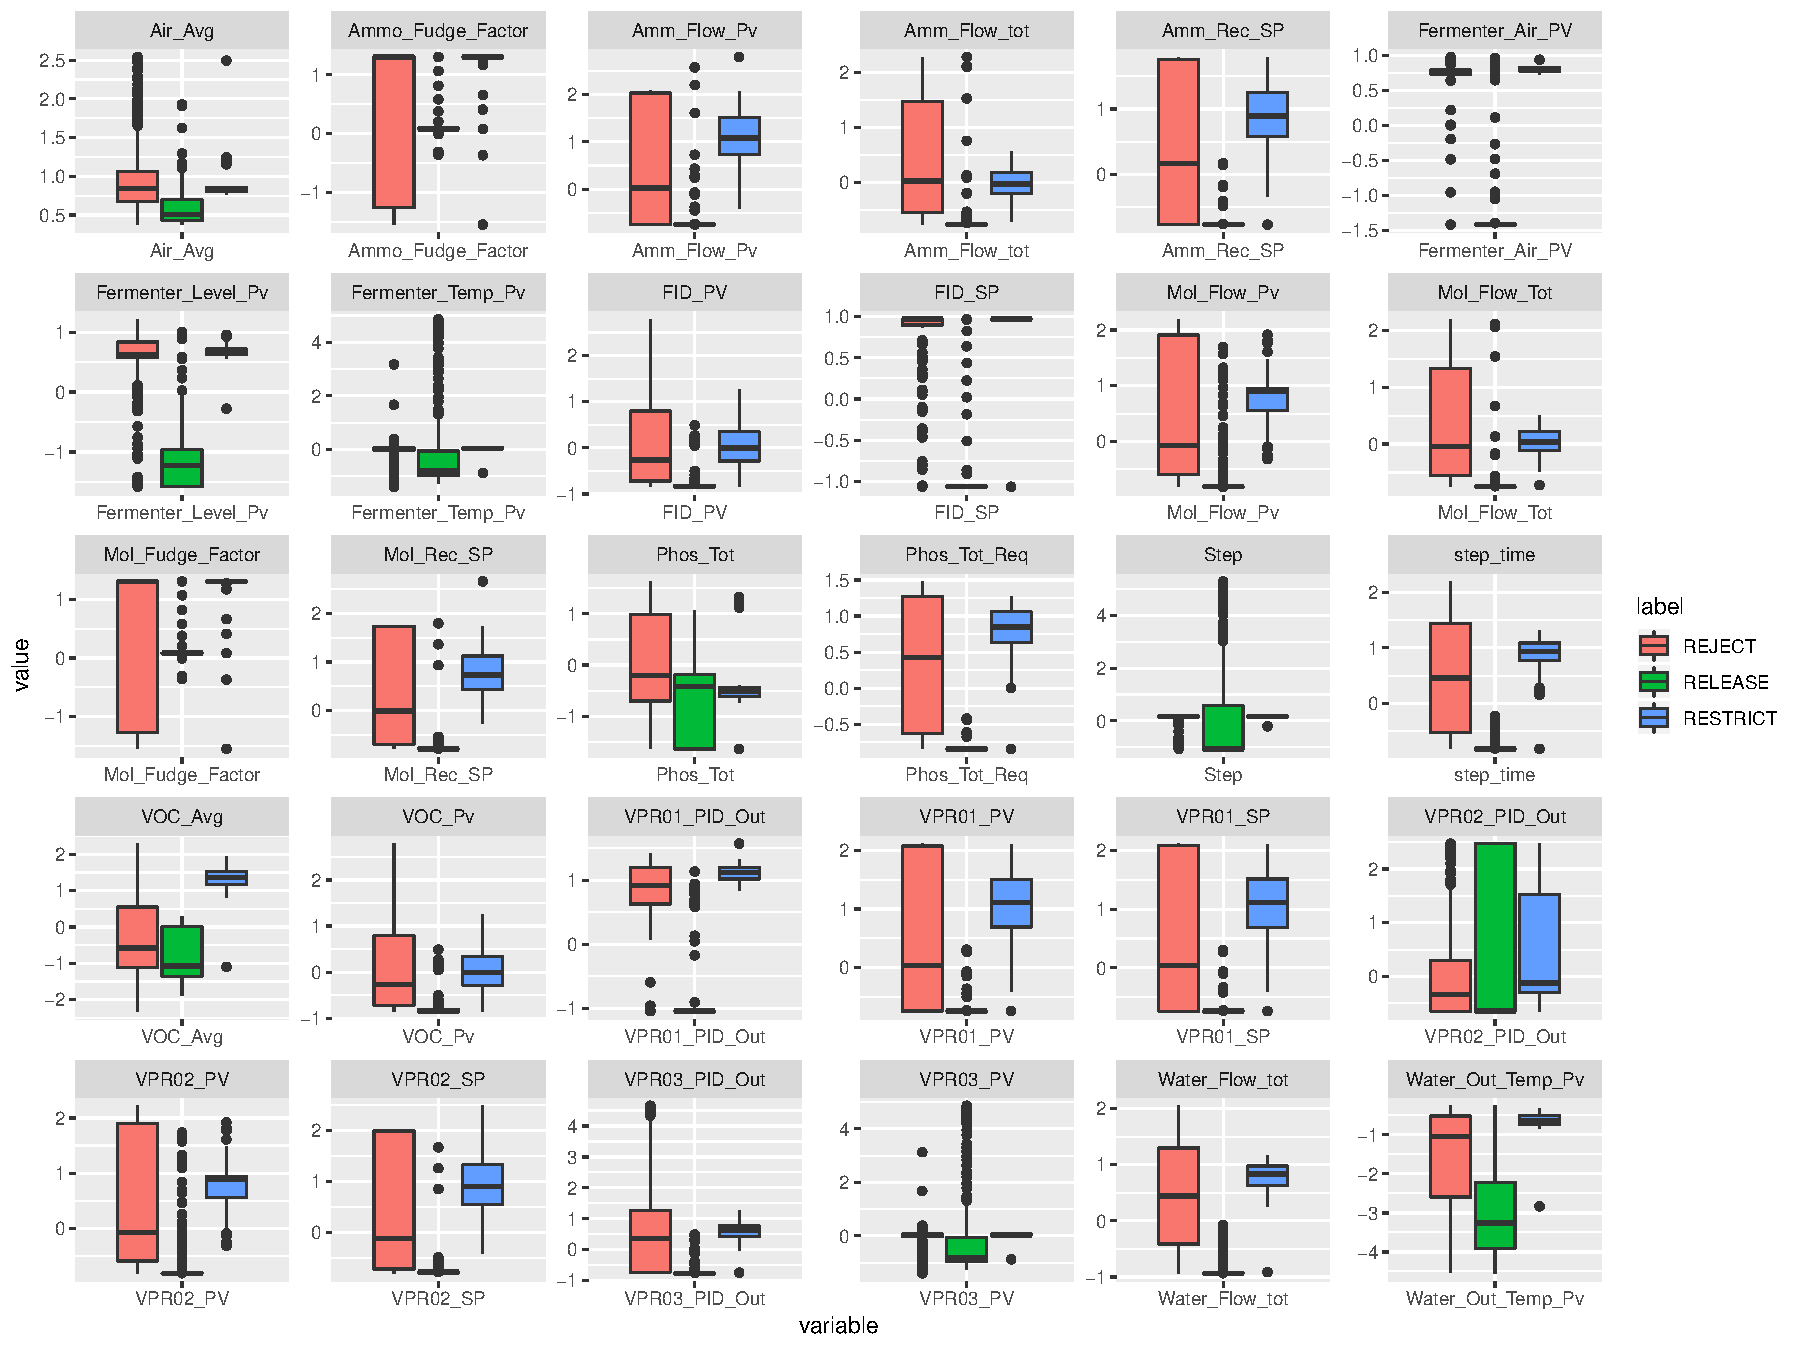
\includegraphics[width=1.0\textwidth]{plots/f2-predicted.pdf}
    \caption{F2 predicted}
    \label{fig:f2_predicted}
\end{figure}

When looking at the effectiveness of feature reduction and clustering, then, as it can be easily seen from Figure \ref{fig:f2_explained_variances}, most of the variance in F2 process data can be explained by one factor, with first 3 factors explaining more than 90\% of the variance in the process data. That indicates that there are strong correlations between parallel time series in the process that can be aggregated into smaller number of series with highly similar explanatory power. Moreover, Figure \ref{fig:f2_variables} also shows a strong clustering indicating correlations and need for feature reduction.

Therefore, when looking only at the feature reduced data and investigating the first, by far, the most significant factor, it is evident, that the ``rejected'' and ``release'' batches are indeed different. See Figure \ref{fig:f2_LD1} for detailed representation. Therefore we believe that the process of F2 should be further investigated.

\begin{figure}[ht!]
    \begin{subfigure}{0.3\textwidth}
        \begin{center}
        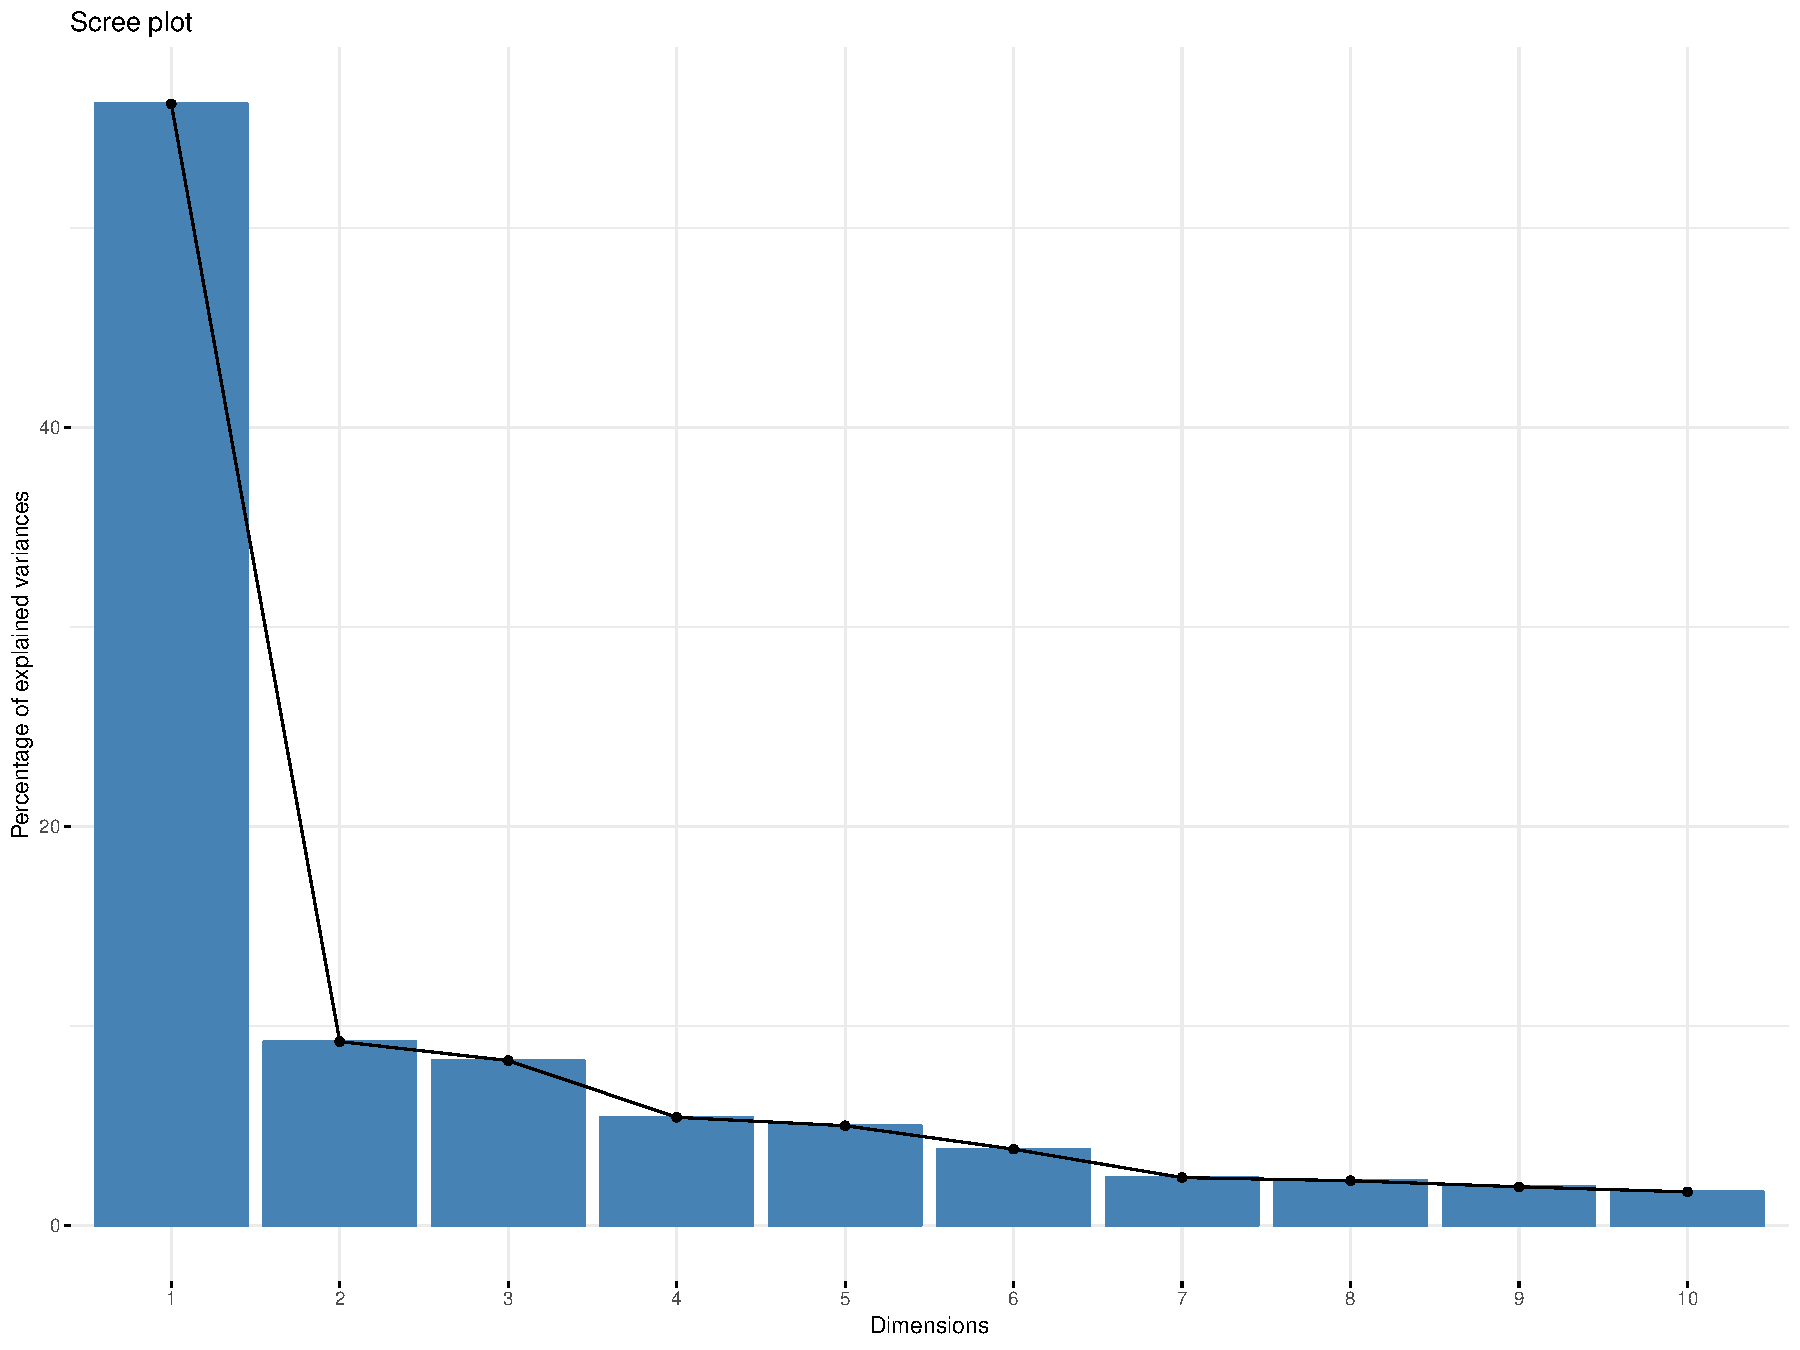
\includegraphics[width=\textwidth]{plots/f2_explained_variances.pdf}       
        \end{center}
        \caption{F2 explained variances}
        \label{fig:f2_explained_variances}
    \end{subfigure}%
    \begin{subfigure}{0.3\textwidth}
        \begin{center}
        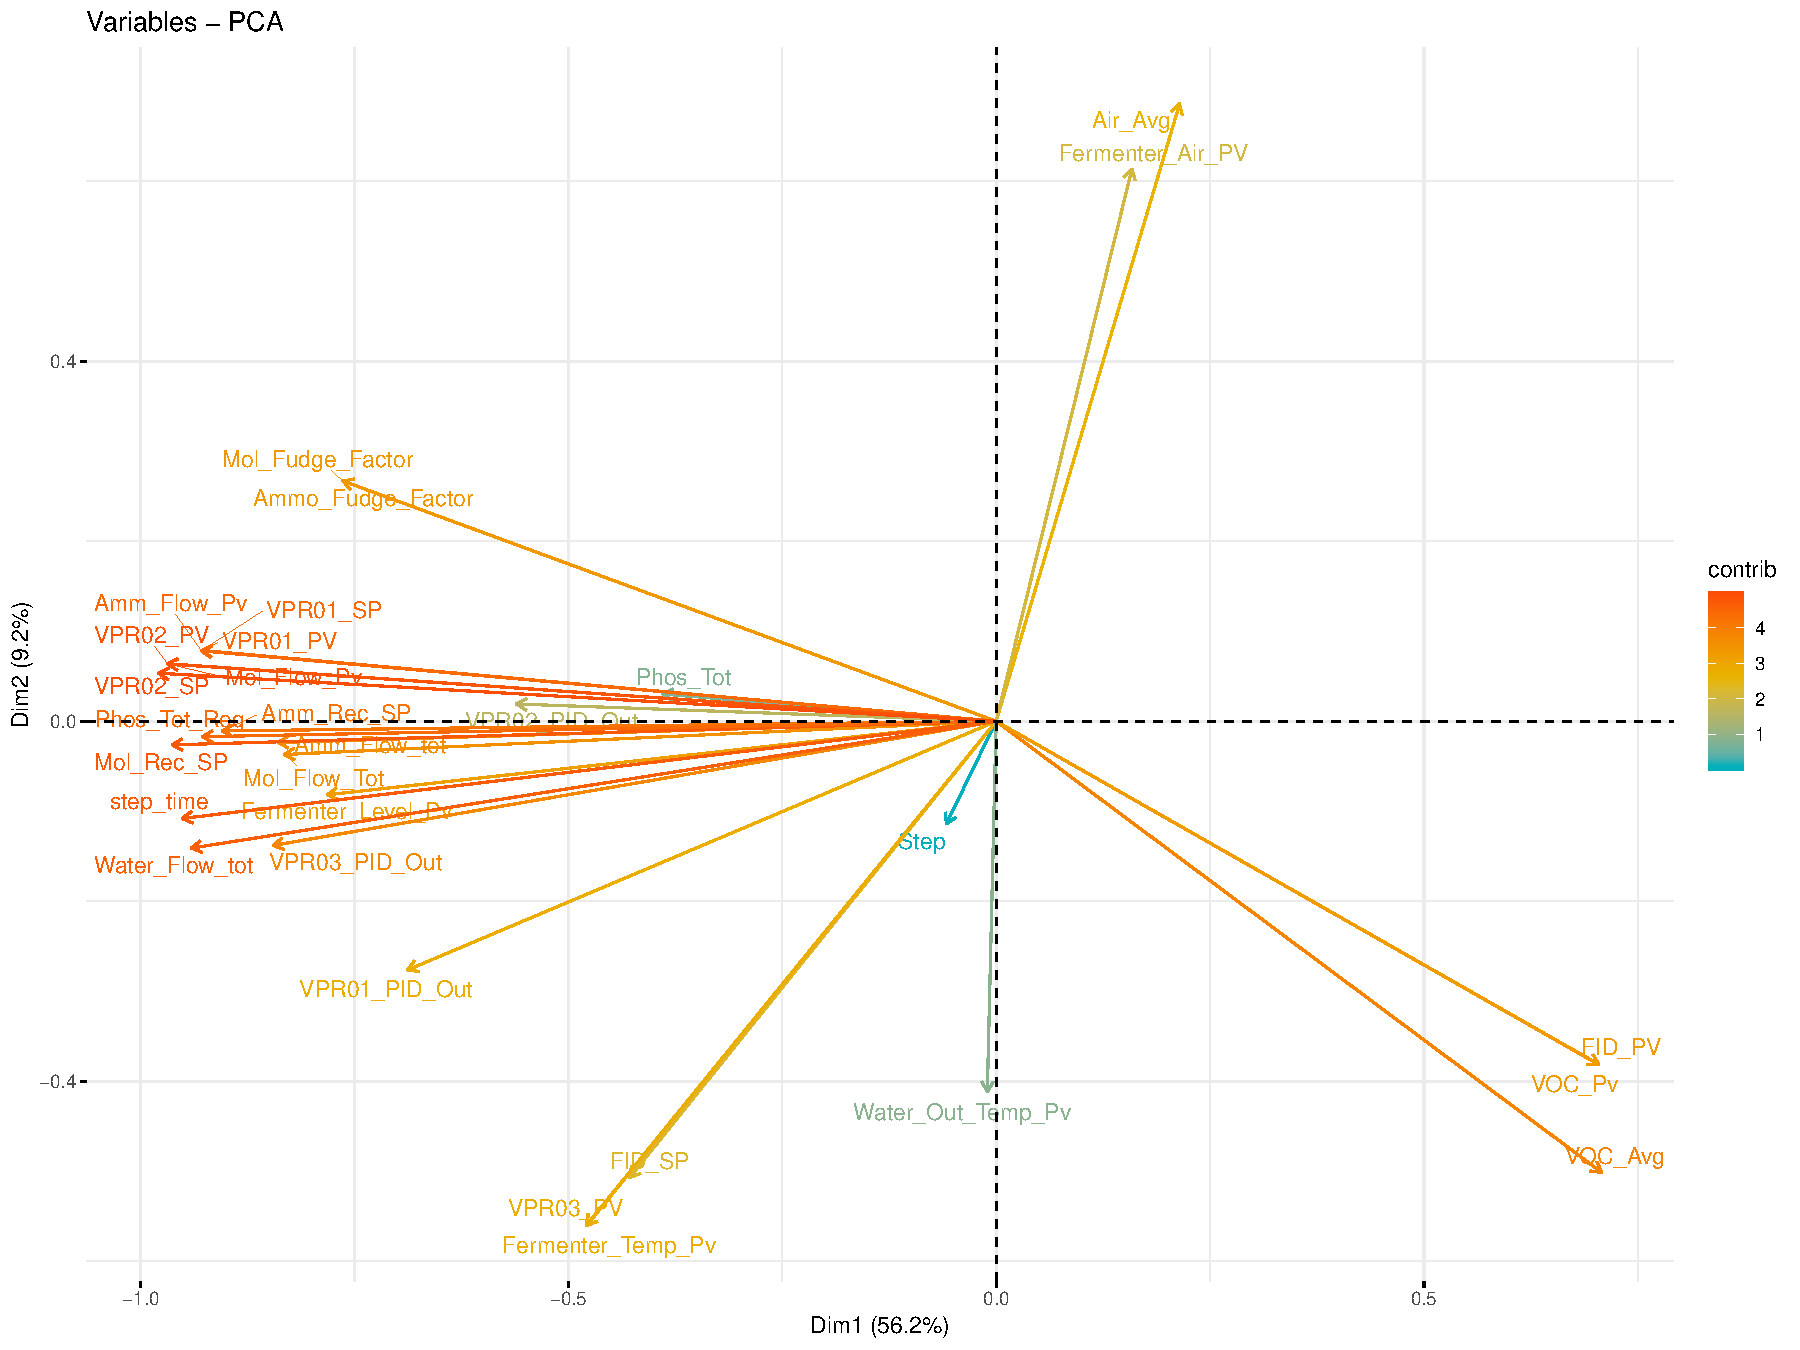
\includegraphics[width=\textwidth]{plots/f2_graph_of_variables.pdf}
        \end{center}
        \caption{F2 Variables}
        \label{fig:f2_variables}
    \end{subfigure}%
    \begin{subfigure}{0.3\textwidth}
        \begin{center}
        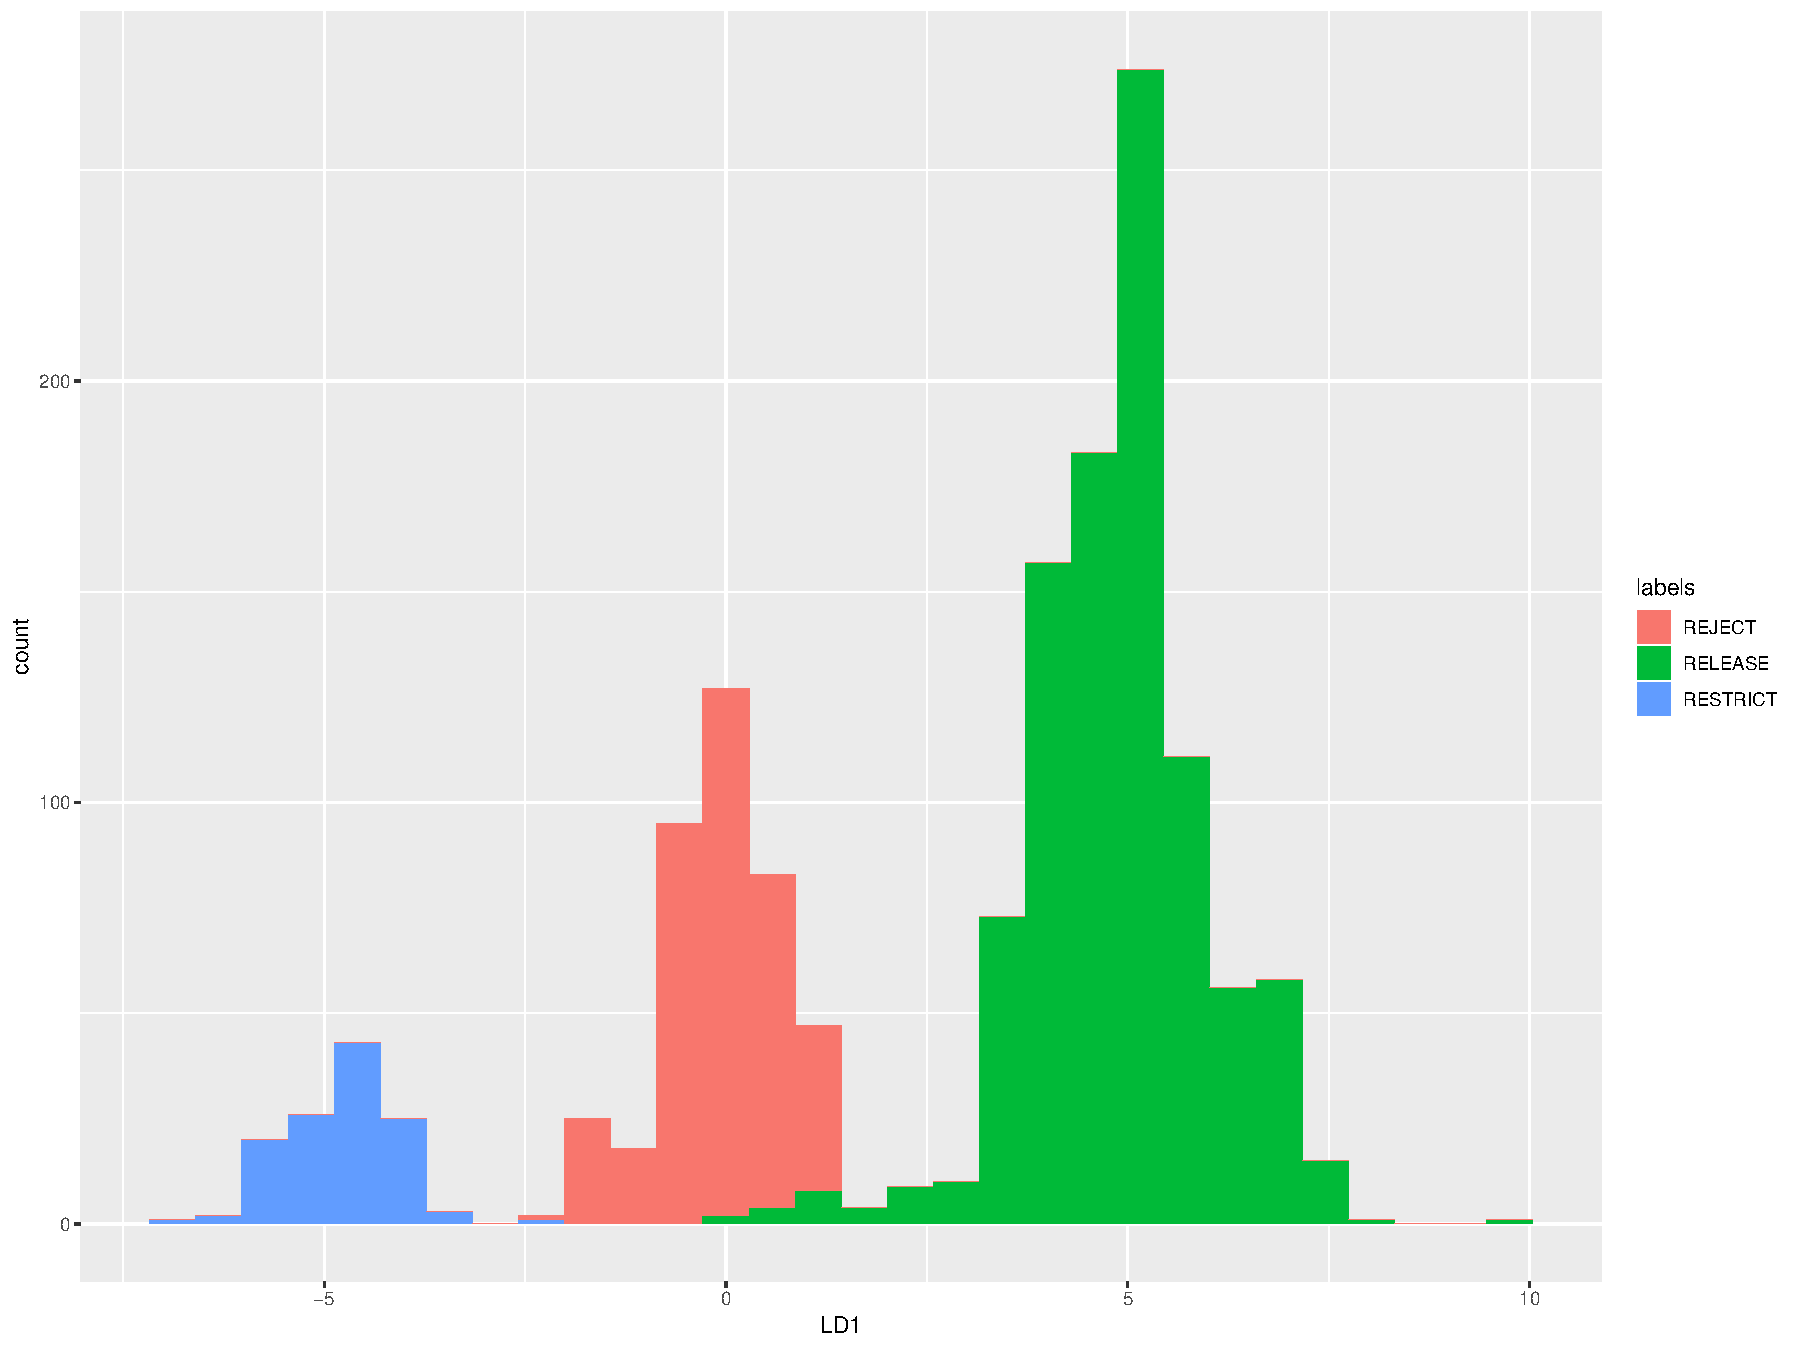
\includegraphics[width=\textwidth]{plots/f2_LD1.pdf}
        \end{center}
        \caption{F2 LD1 distribution across classes}
        \label{fig:f2_LD1}
    \end{subfigure}
    \caption{F2 component analysis}
\end{figure}


\subsection{Analysis of F4}
The analysis of step F4 was performed similarly to the step F2 above. We investigated the variance of data to see the potential differences between the classes. Then we performed PCA and LDA to investigate the clustering of the data and to see whether the differences between the clusters are indeed significant.

Compared to F5, F4 was relatively well populated data set. Again, the main weakness lies within the uneven balance between ``released'' and ``rejected'' classes. Therefore, the conclusions and results of the analysis are statistically weak and either need to be improved by additional data collection and experimentation of significant injection of process knowledge. As it is evident from the box plot of the data depicted on Figure \ref{fig:f4_sample}, the difference between three classes of batches appears to be insignificant. Most medians of the time series are close to each other and the variance of the 25\% and 75\% percentiles can be explained by a few number of random observations that have shifted the percentile cutoff points. 

\begin{figure}[ht!]
    \centering
    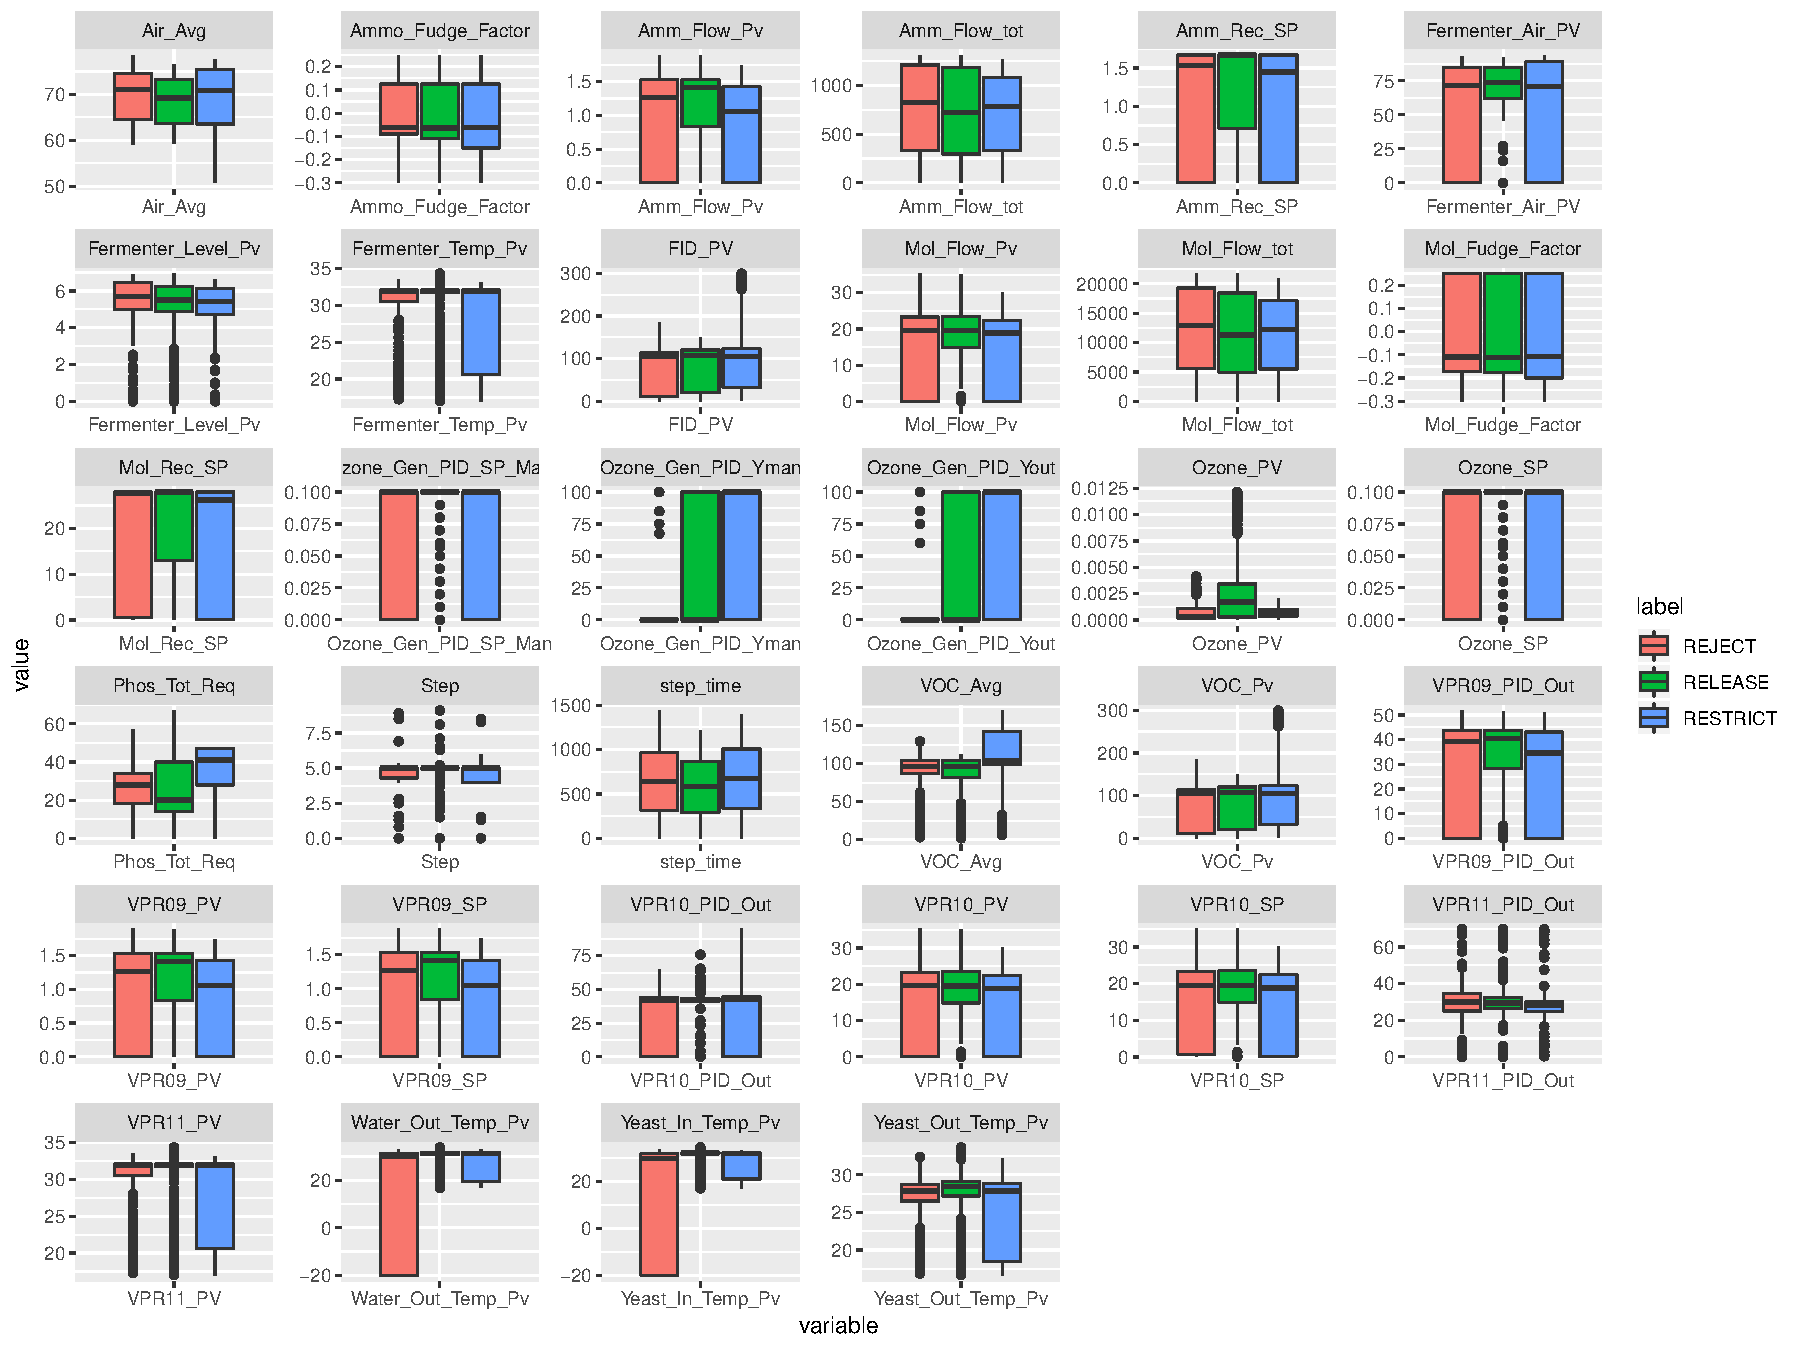
\includegraphics[width=1.0\textwidth]{plots/f4-sample.pdf}
    \caption{F4 sample}
    \label{fig:f4_sample}
\end{figure}

Similar picture can be seen with modelled data and predicted labels shown at Figure \ref{fig:f4_predicted}, no significant difference exists, the only differentiator here compared to the previous figure is, that due to the similarity, the predictive power of the model is low and thus the data points have received erroneous labels from the model with a significant amount of ``rejected'' category data points being labelled as ``released''.

\begin{figure}[ht!]
    \centering
    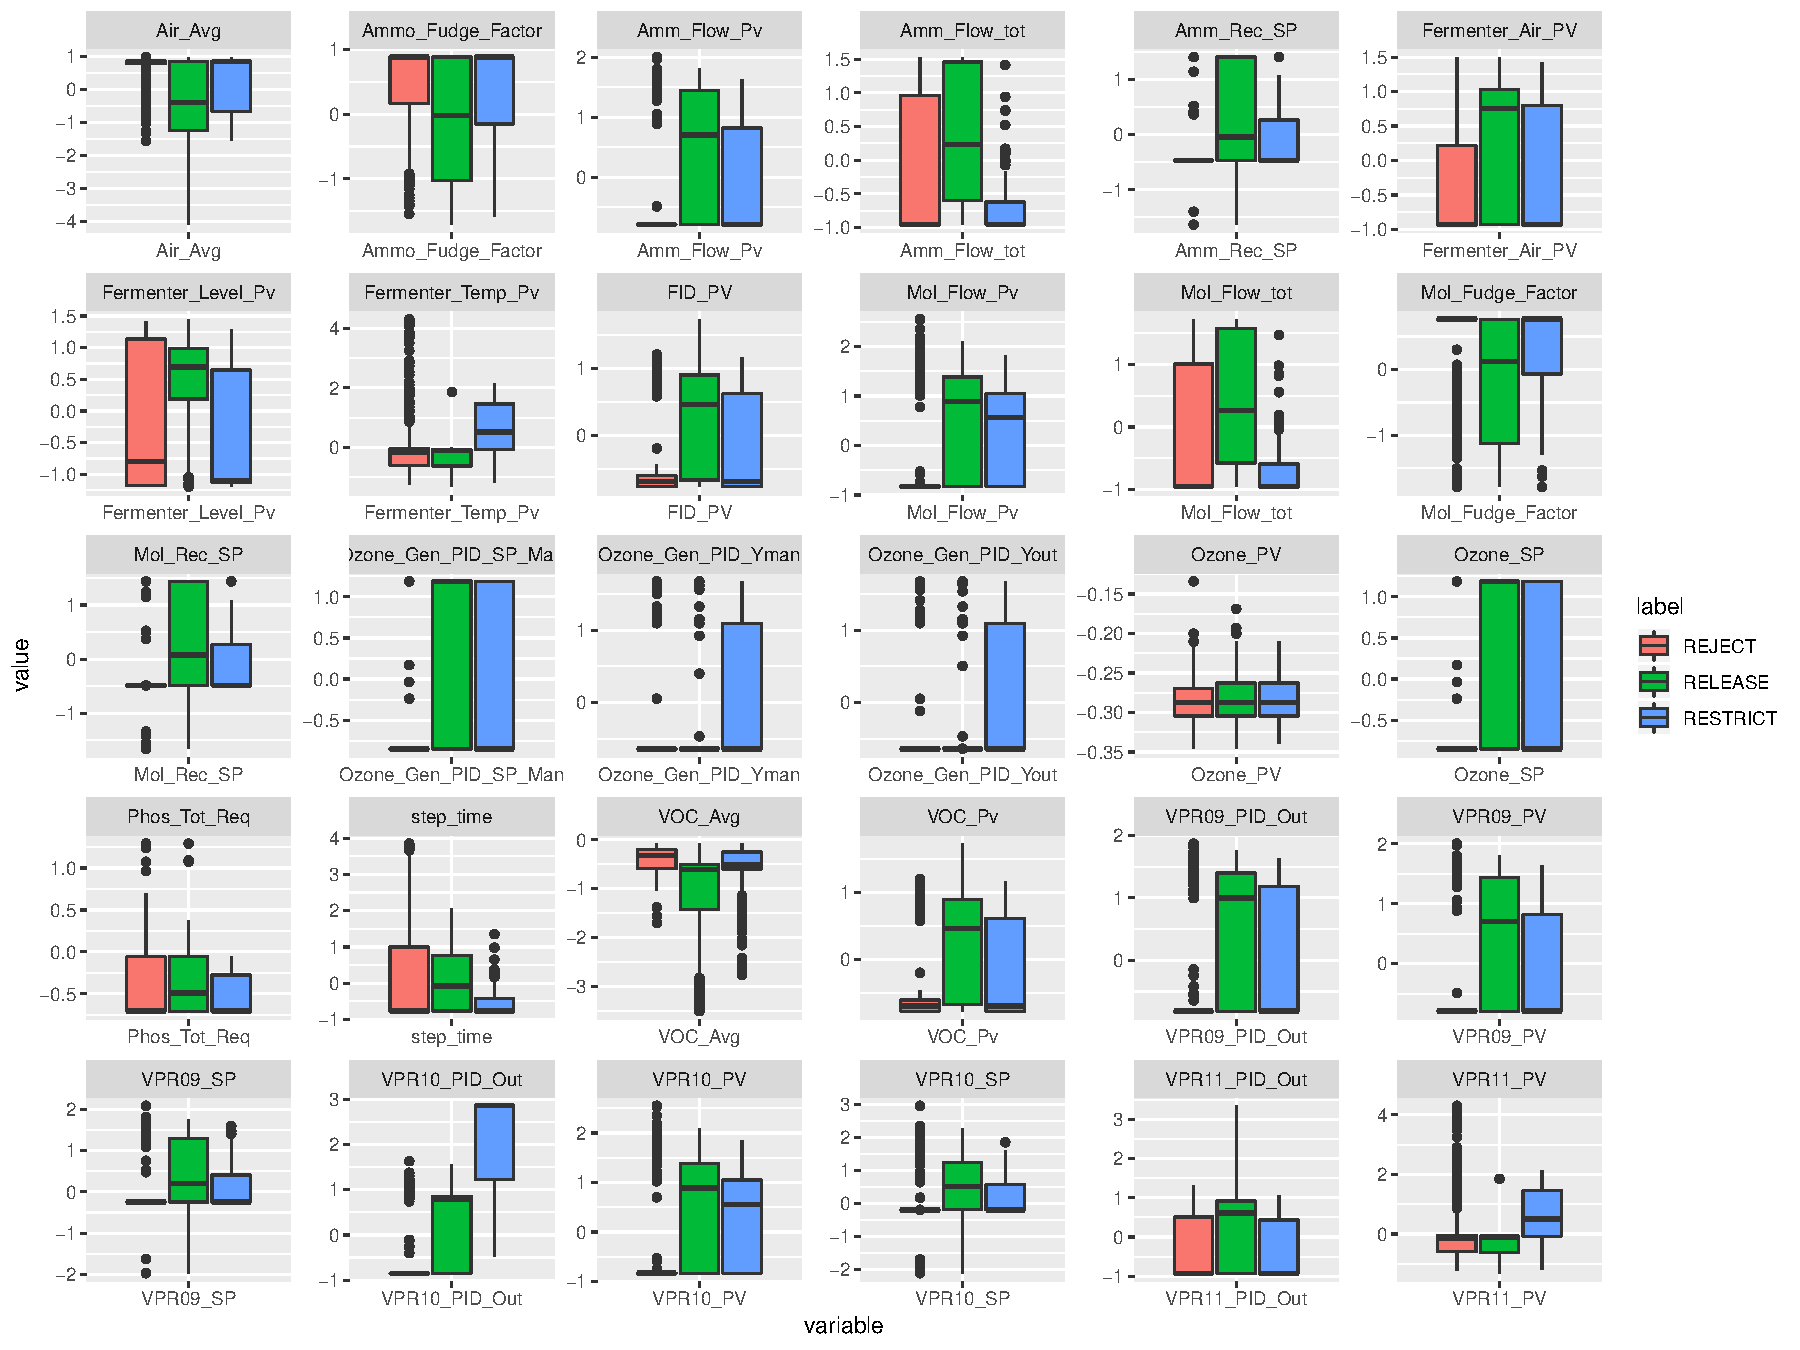
\includegraphics[width=1.0\textwidth]{plots/f4-predicted.pdf}
    \caption{F4 predicted}
    \label{fig:f4_predicted}
\end{figure}

When looking at the results of PCA and LDA, then the results of PCA are significant. Again, due to strong correlations between parallel time series, the data can be significantly feature reduced. The effect of PCA as displayed on Figure \ref{fig:f4_explained_variances} is significant, with first 3 components explaining well over 90\% of the variance in the time series. That, similarly to F2, is supported by strong clustering of process variables as evident on Figure \ref{fig:f4_variables}. Correlations between the time series create one significant cluster (LD1 axis positive values) and two smaller clusters in $3^{rd}$ and $4^{th}$ quadrants of the chart.

\begin{figure}[ht!]
    \begin{subfigure}{0.3\textwidth}
        \begin{center}
            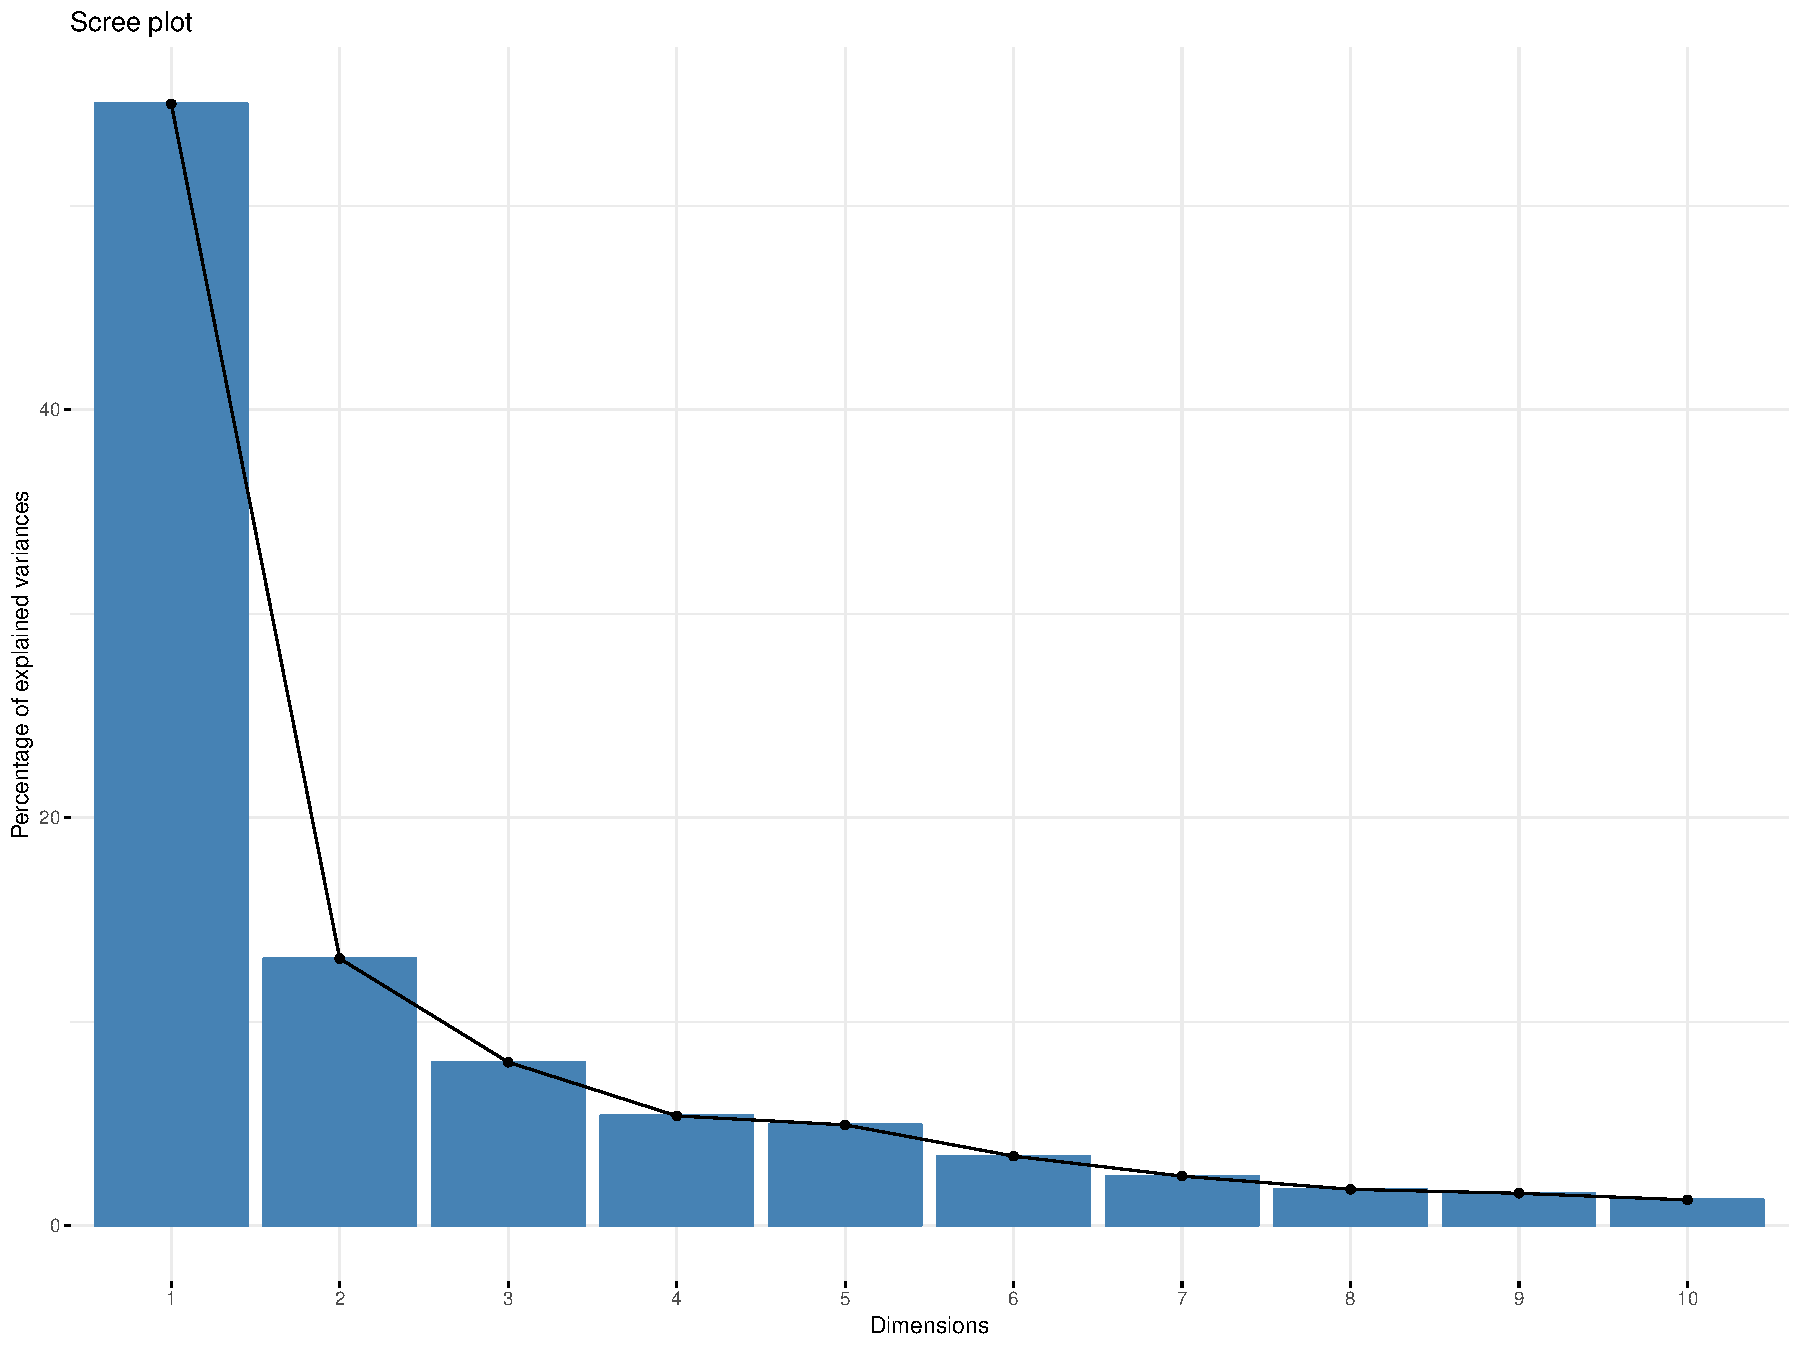
\includegraphics[width=\textwidth]{plots/f4_explained_variances.pdf}        
        \end{center}
        \caption{F4 explained variances}
        \label{fig:f4_explained_variances}
    \end{subfigure}%
    \begin{subfigure}{0.3\textwidth}
        \begin{center}
        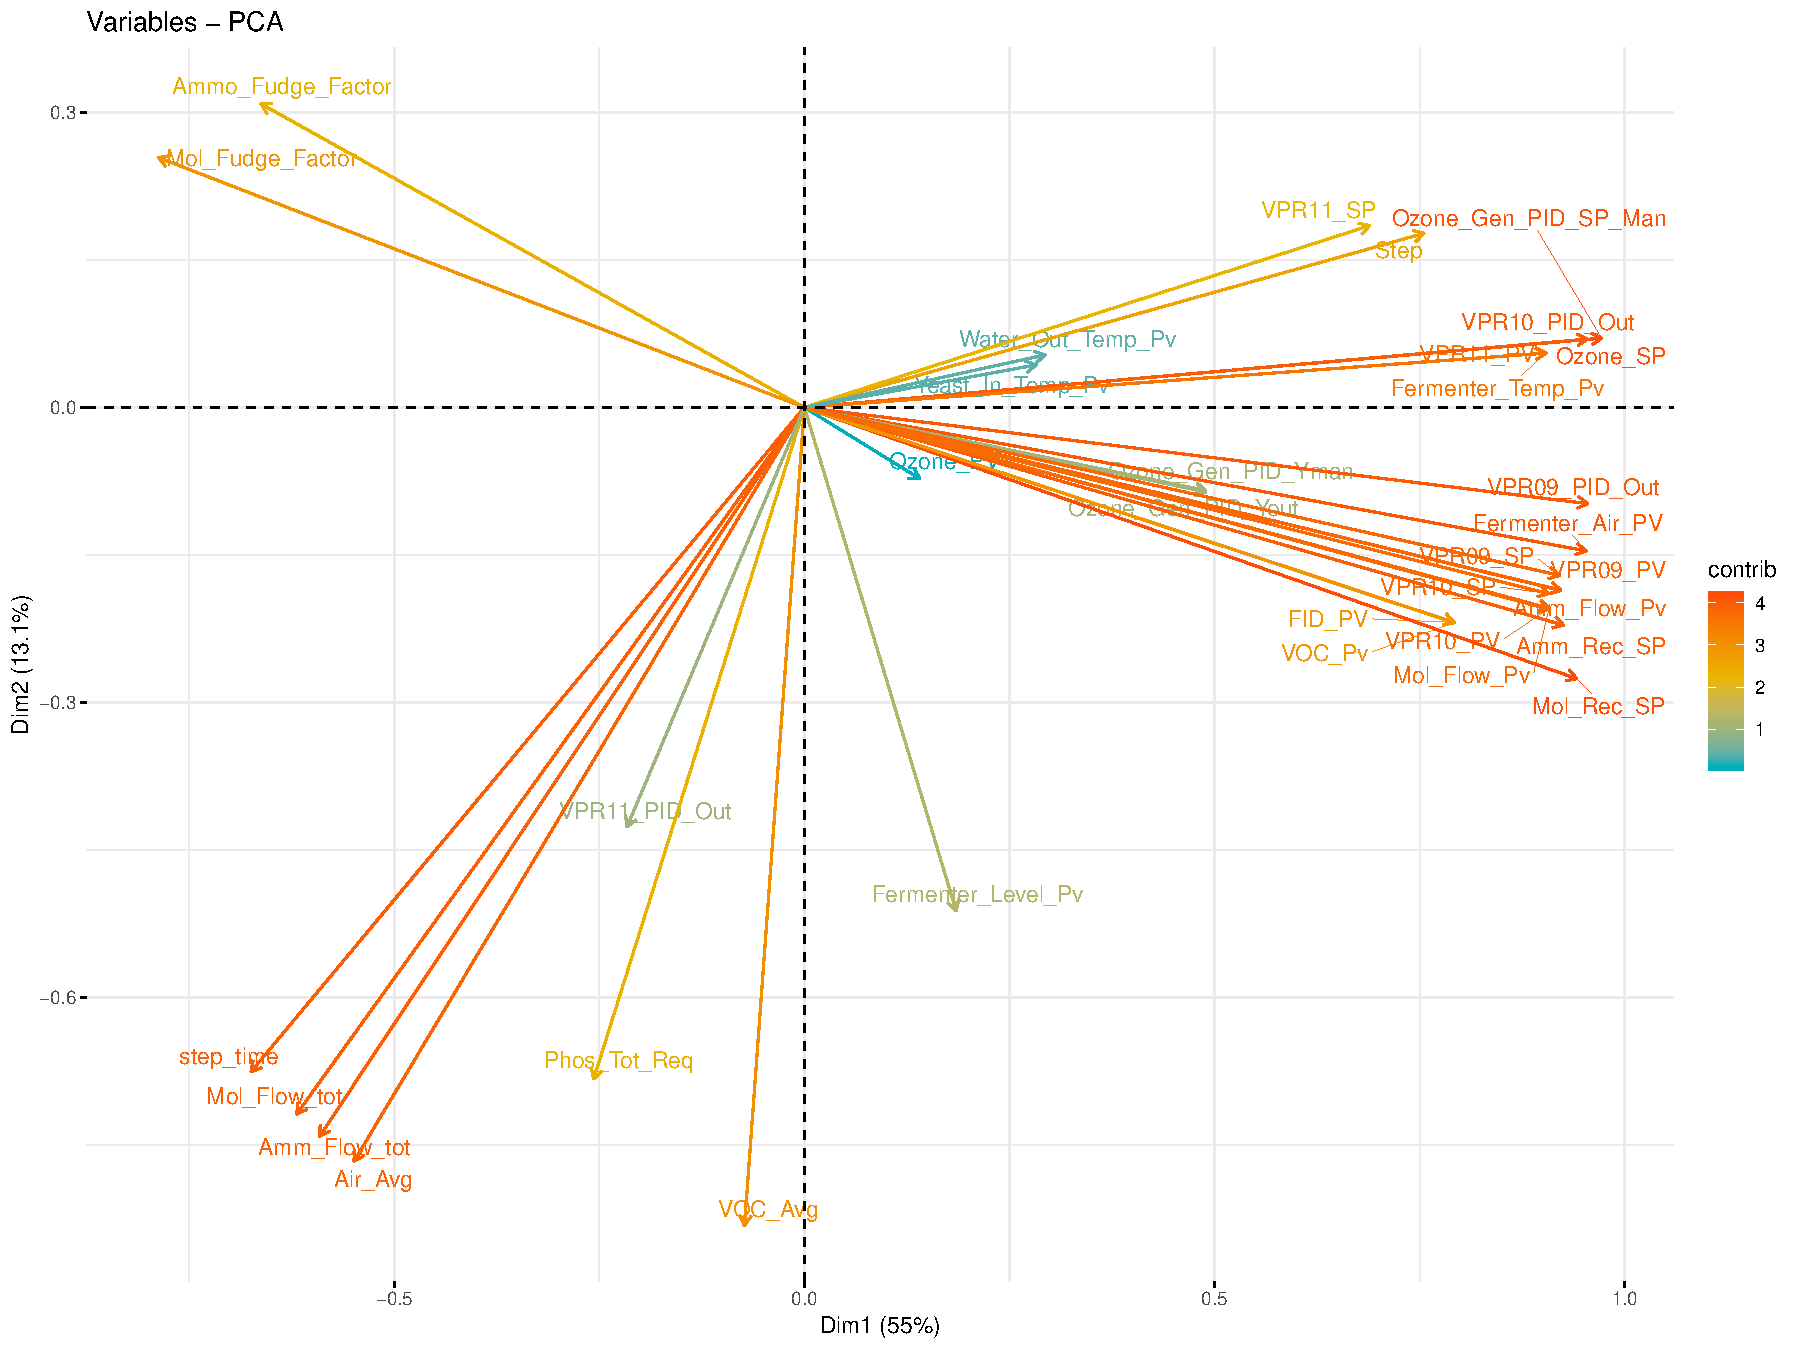
\includegraphics[width=\textwidth]{plots/f4_graph_of_variables.pdf}
        \end{center}
        \caption{F4 Variables}
        \label{fig:f4_variables}
    \end{subfigure}%
    \begin{subfigure}{0.3\textwidth}
        \begin{center}
        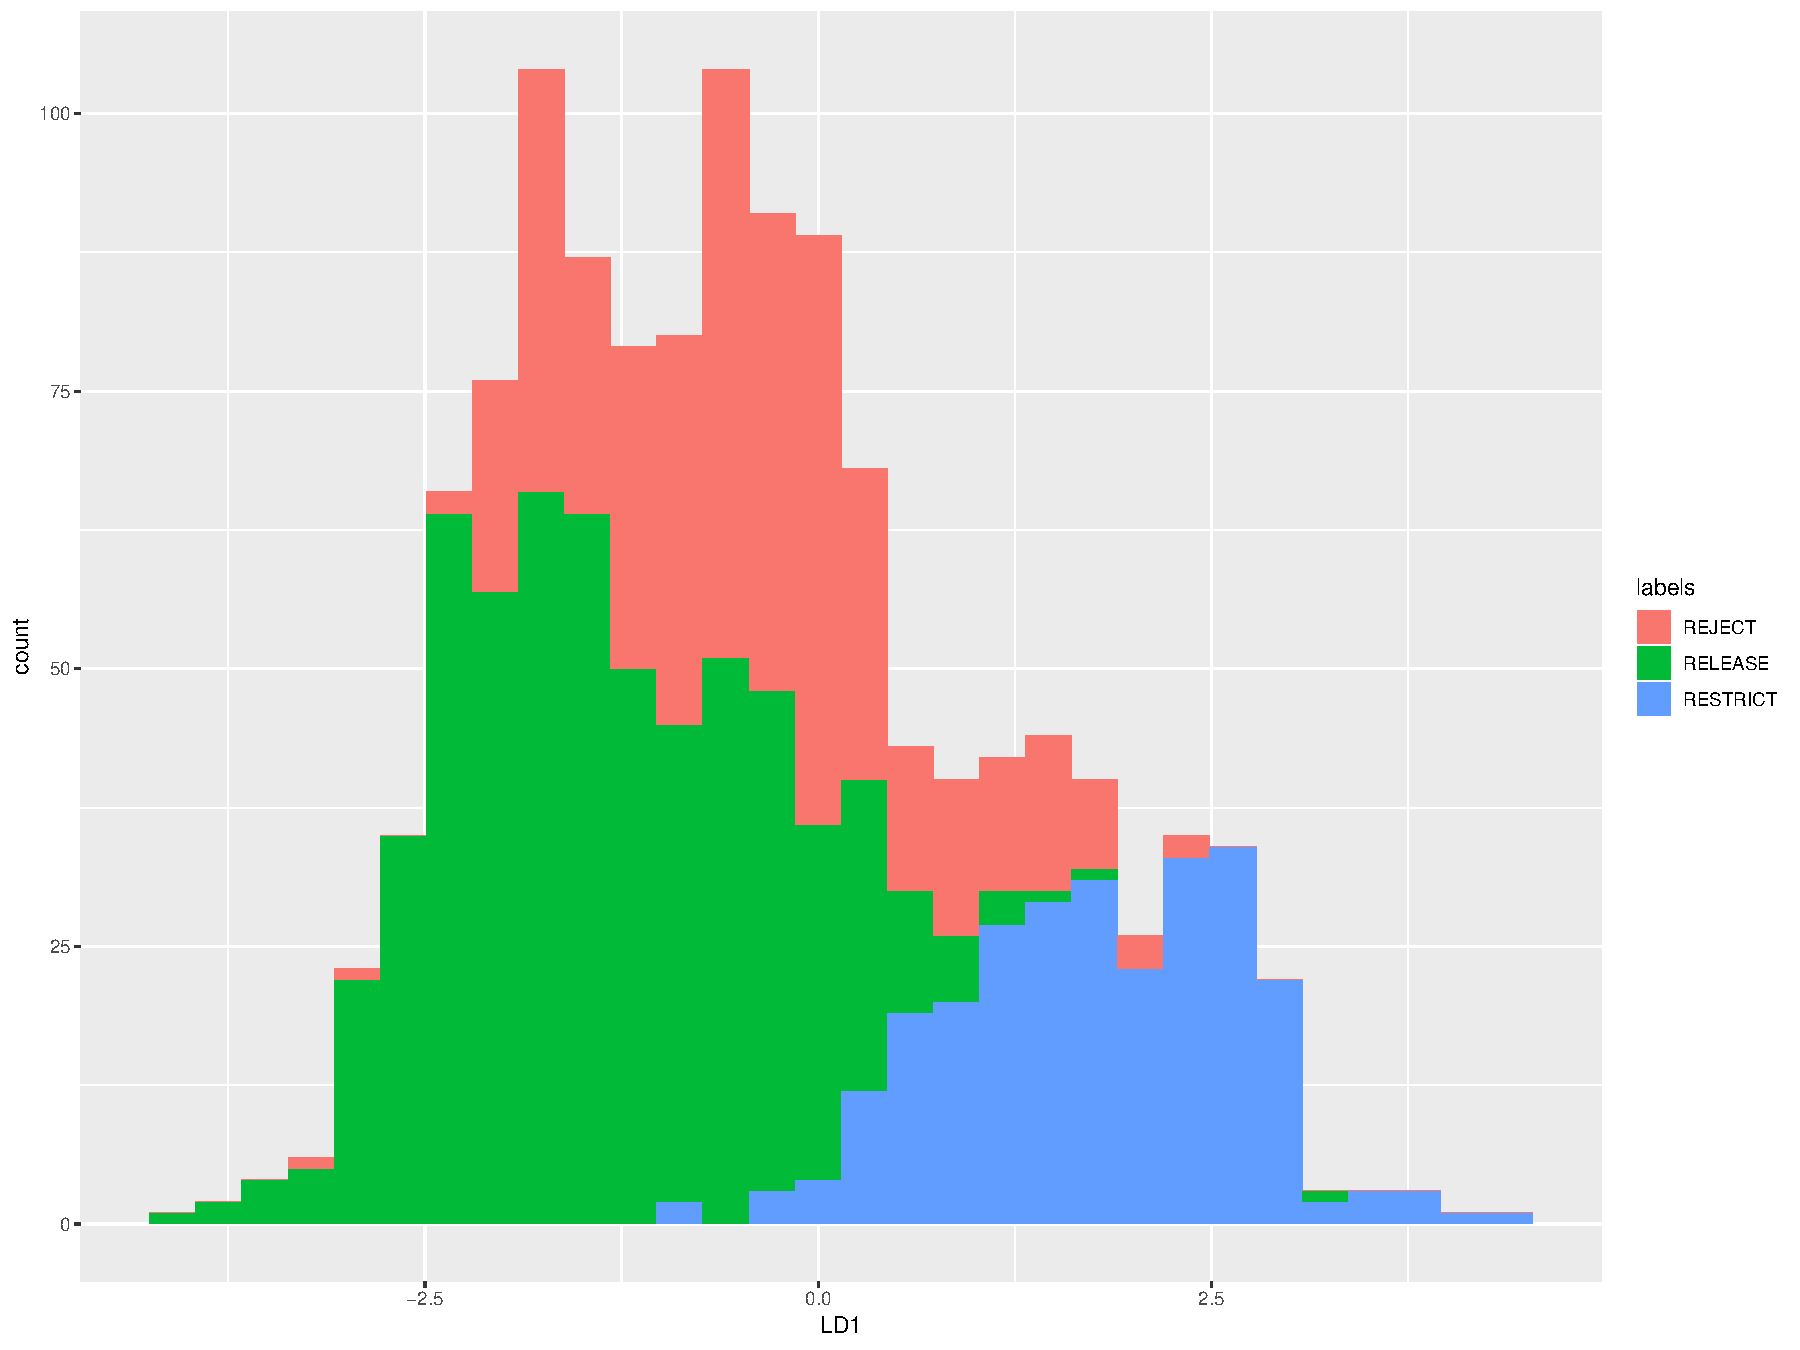
\includegraphics[width=\textwidth]{plots/f4_LD1.pdf}
        \end{center}
        \caption{F4 LD1 distribution across classes}
        \label{fig:f4_LD1}
    \end{subfigure}
    \caption{F4 component analysis}
\end{figure}

Nevertheless, LDA clustering was able to differentiate poorly between the three classes of batches as can be seen on Figure \ref{fig:f2_LD1}. It should be noted, that since the sample sizes are low, the differentiation can be random, ie. the LDA shows significant difference, because for whatever reason (environment, randomness, other nuisance factors) a few batches have different parametric data because the automation and process control system has behaved differently. Additional data and process knowledge are obviously needed before making and in-depth conclusions.

\clearpage
\subsection{Analysis of F5}
Lastly we performed the same analysis steps on F5. Before going any further, it should be noted, that since we had only two samples in F5 - one rejected and one release, then the results of the analysis are far for conclusive, lack strong statistical significance and are indicative at best. 

As it can be seen from box plots at Figure \ref{fig:f5_sample}, the process data with its medians, 25\% and 75\% percentiles varying with no clear pattern. Again, as with analysis of F2 and F4, the plot does not depict time series that were either constant or otherwise lacking explanatory information. It should be noted, that there is an interesting behaviour regarding air (\texttt{Air\_PID\_Out} and \texttt{Air\_PV}), ammonia (\texttt{Amm\_Flow\_Tot}) and molasses (\texttt{Mol\_Flow\_Tot}). 

\begin{figure}[ht!]
    \centering
    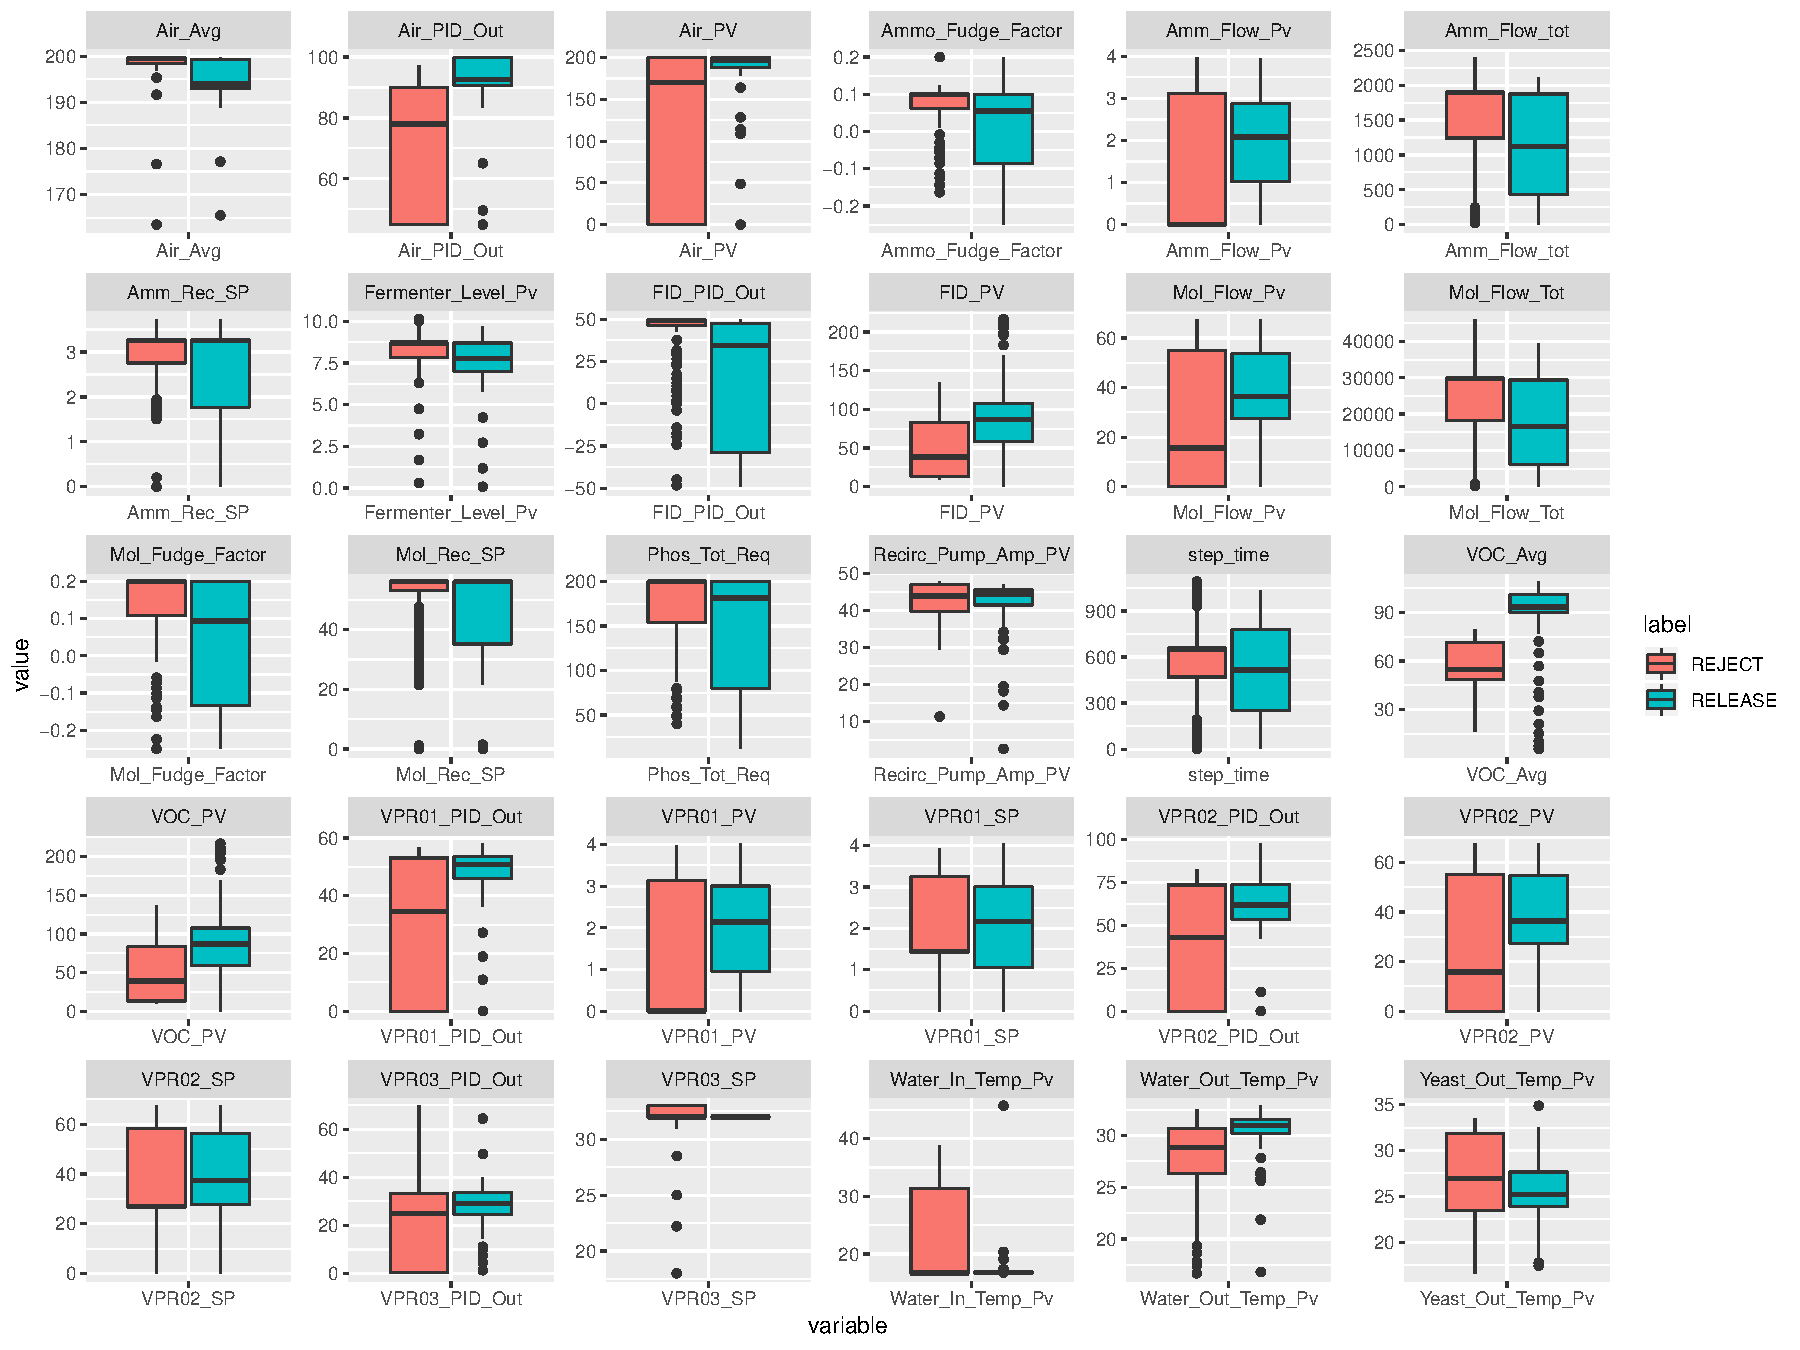
\includegraphics[width=1.0\textwidth]{plots/f5-sample.pdf}
    \caption{F5 sample}
    \label{fig:f5_sample}
\end{figure}

\begin{figure}[ht!]
    \centering
    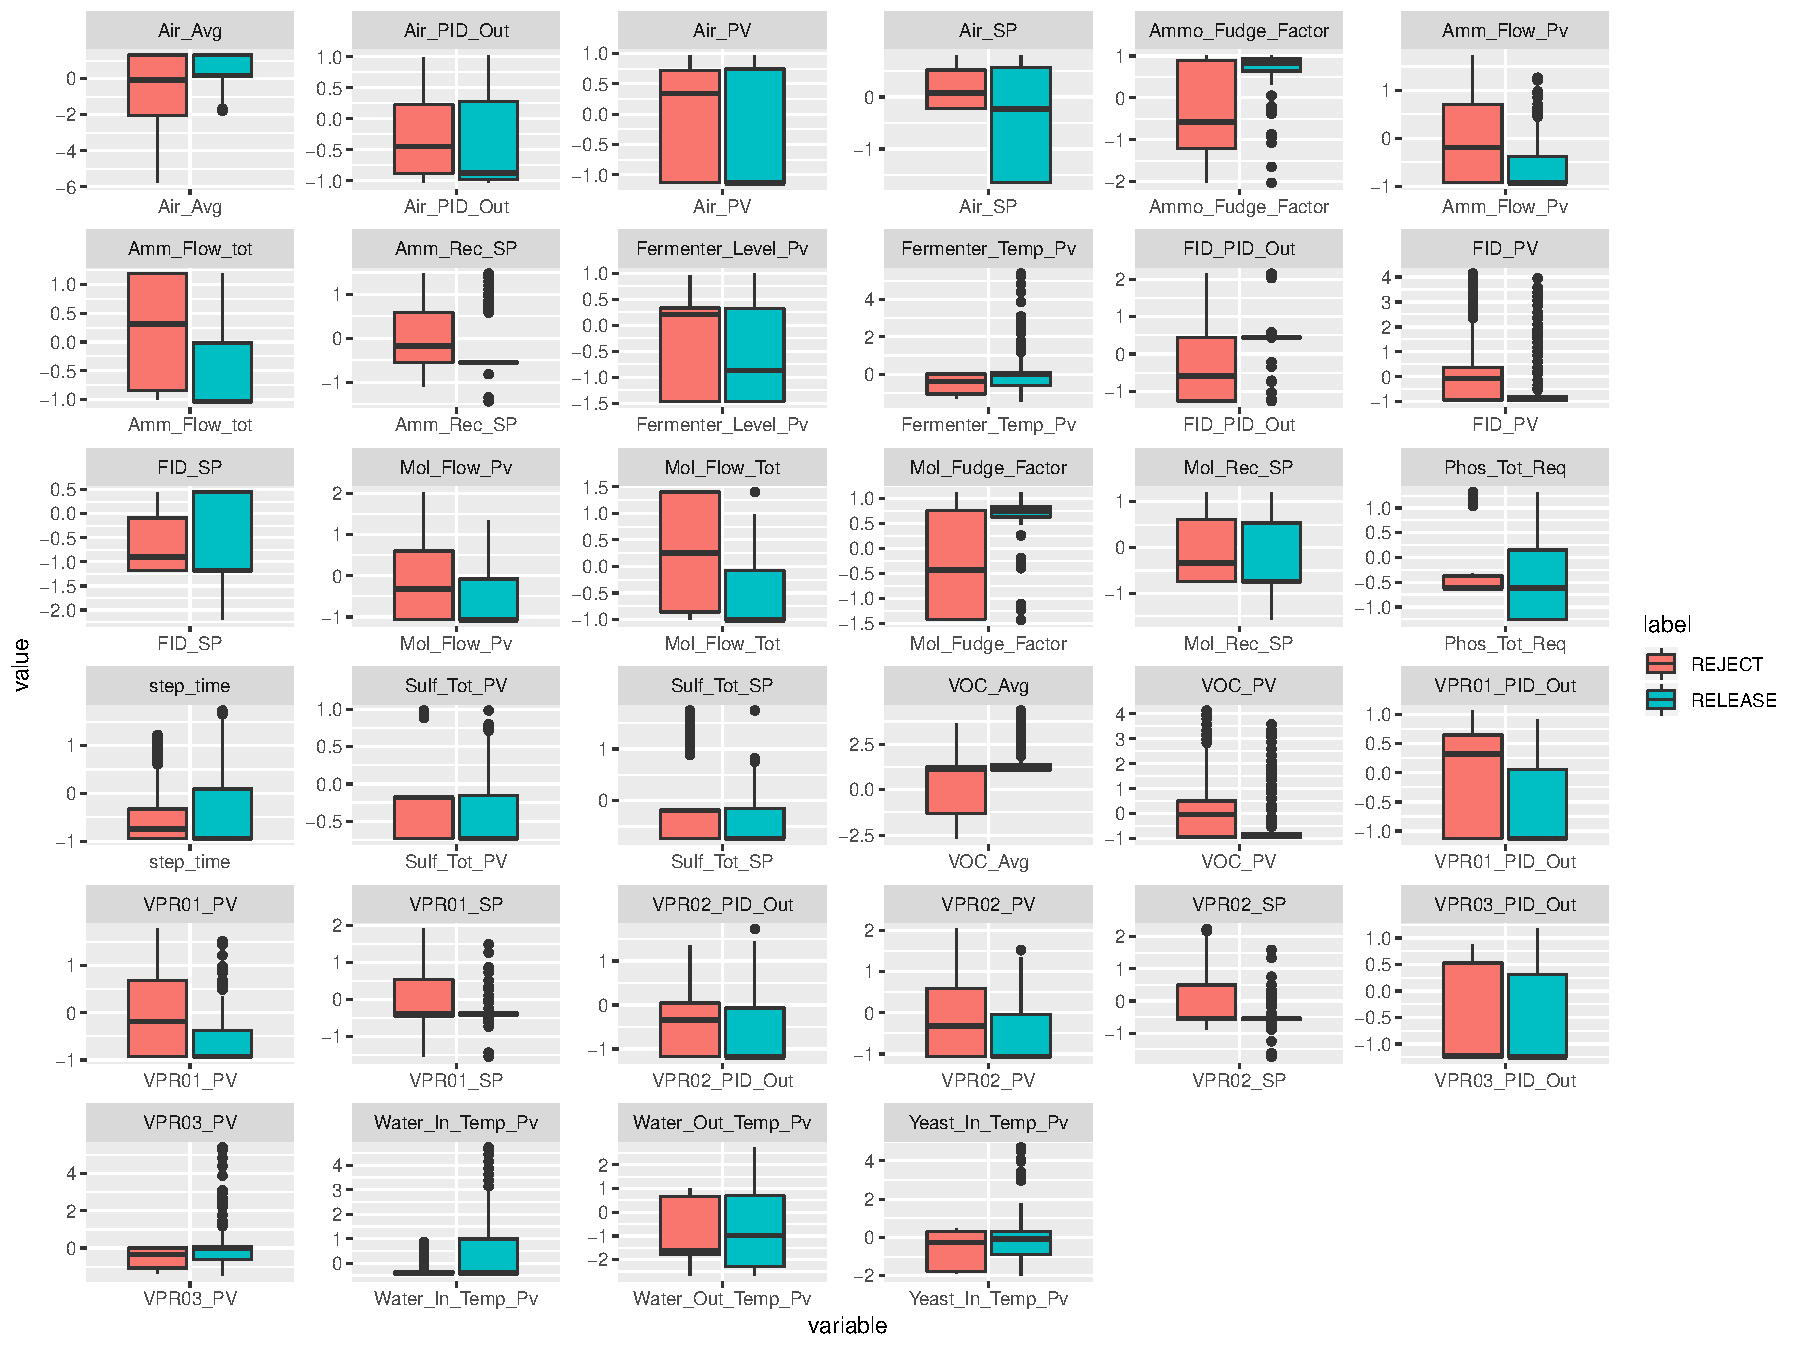
\includegraphics[width=1.0\textwidth]{plots/f5-predicted.pdf}
    \caption{F5 predicted}
    \label{fig:f5_predicted}
\end{figure}

After performing the feature reduction and cluster analysis (PCA and LDA respectively), the lack of data was again evident. When investigating the effectiveness of feature reduction (see Figure \ref{fig:f5_variables}) then, clustering of variables, albeit present, is weak. 

\begin{figure}[ht!]
    \centering
    \begin{subfigure}{.3\textwidth}
        \centering
        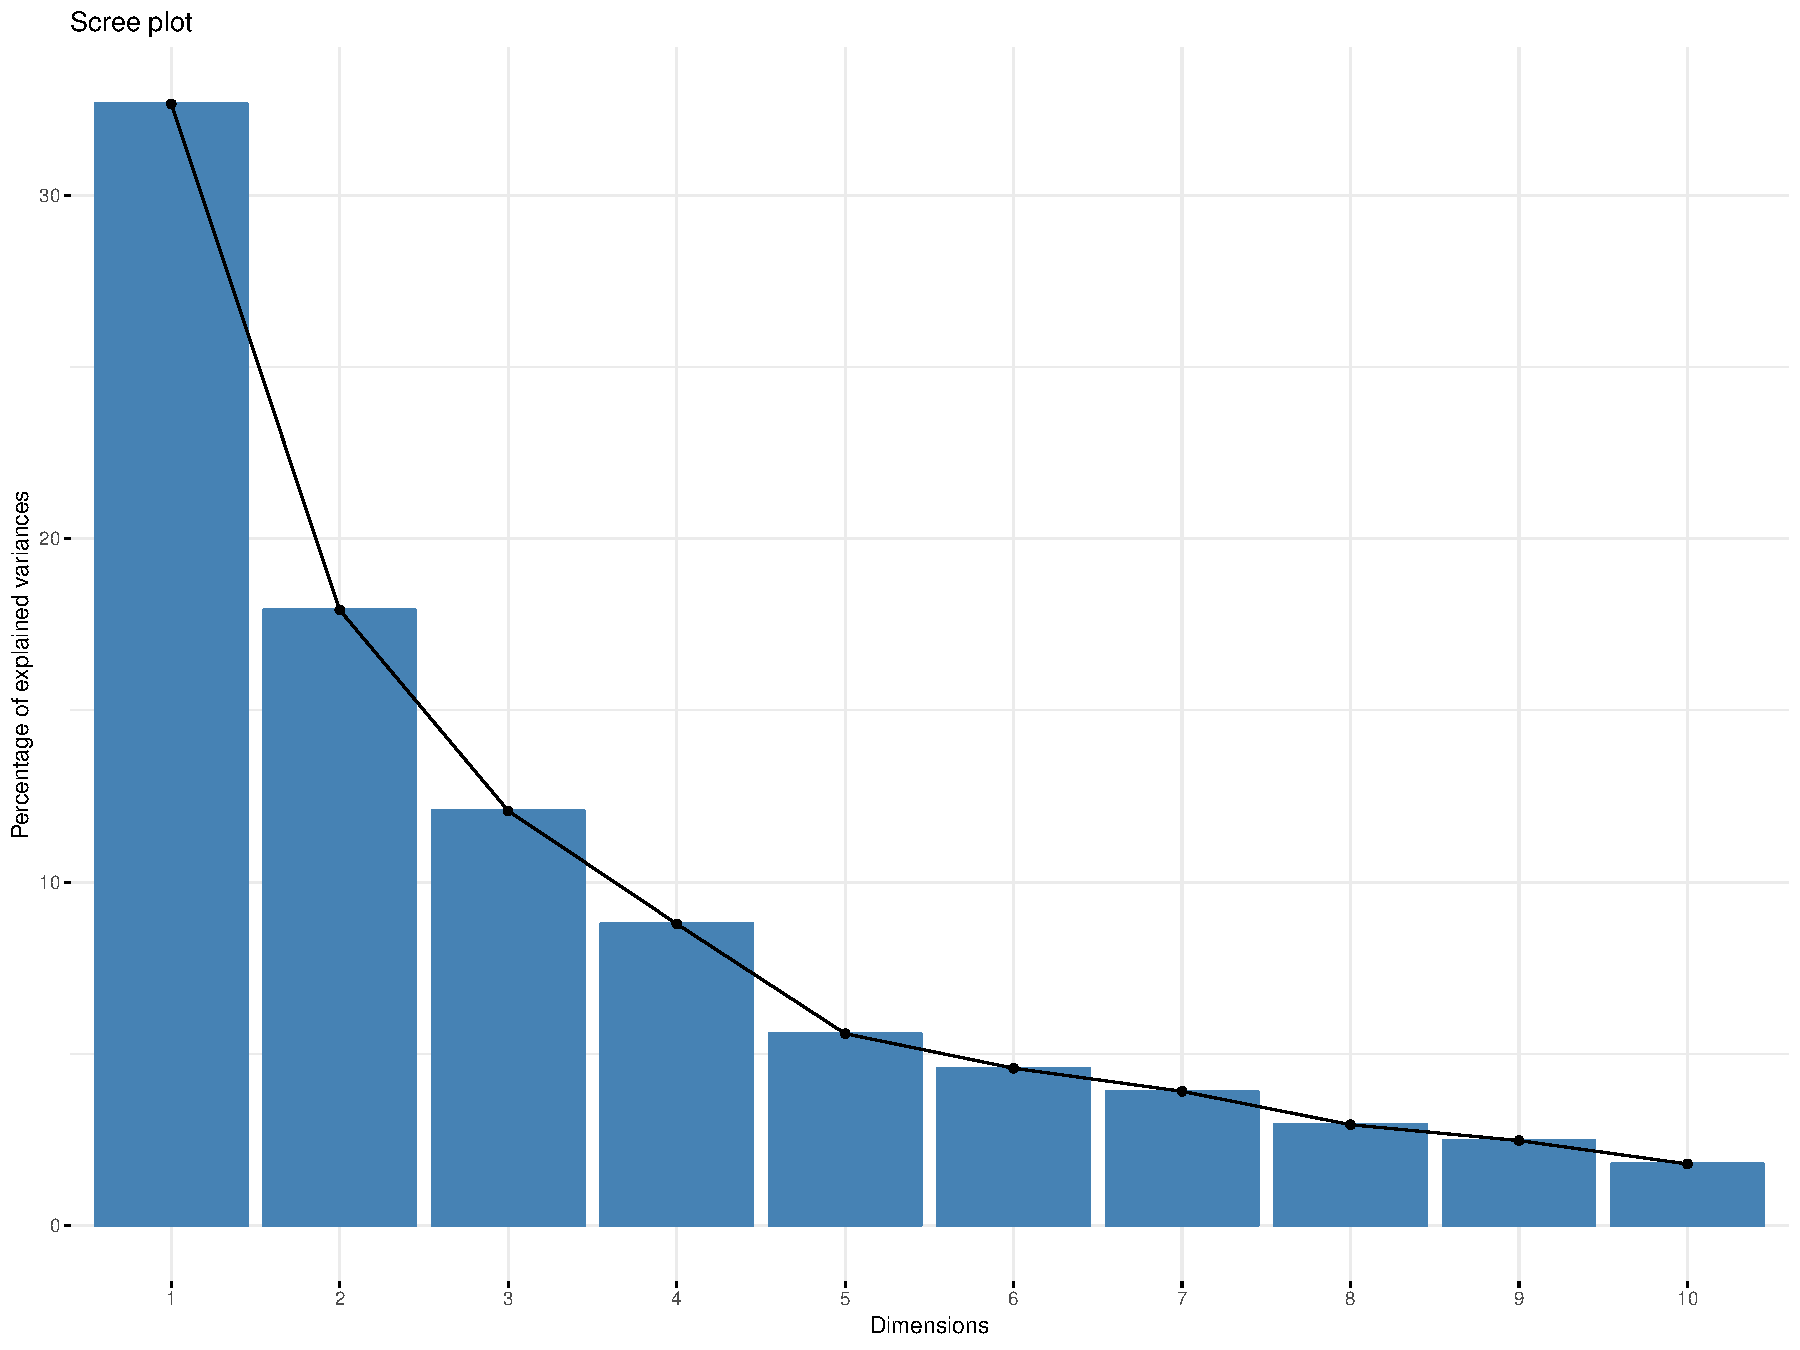
\includegraphics[width=\textwidth]{plots/f5_explained_variances.pdf}        
        \caption{F5 explained variances}
        \label{fig:f5_explained_variances}
    \end{subfigure}%
    \begin{subfigure}{.3\textwidth}
        \centering
        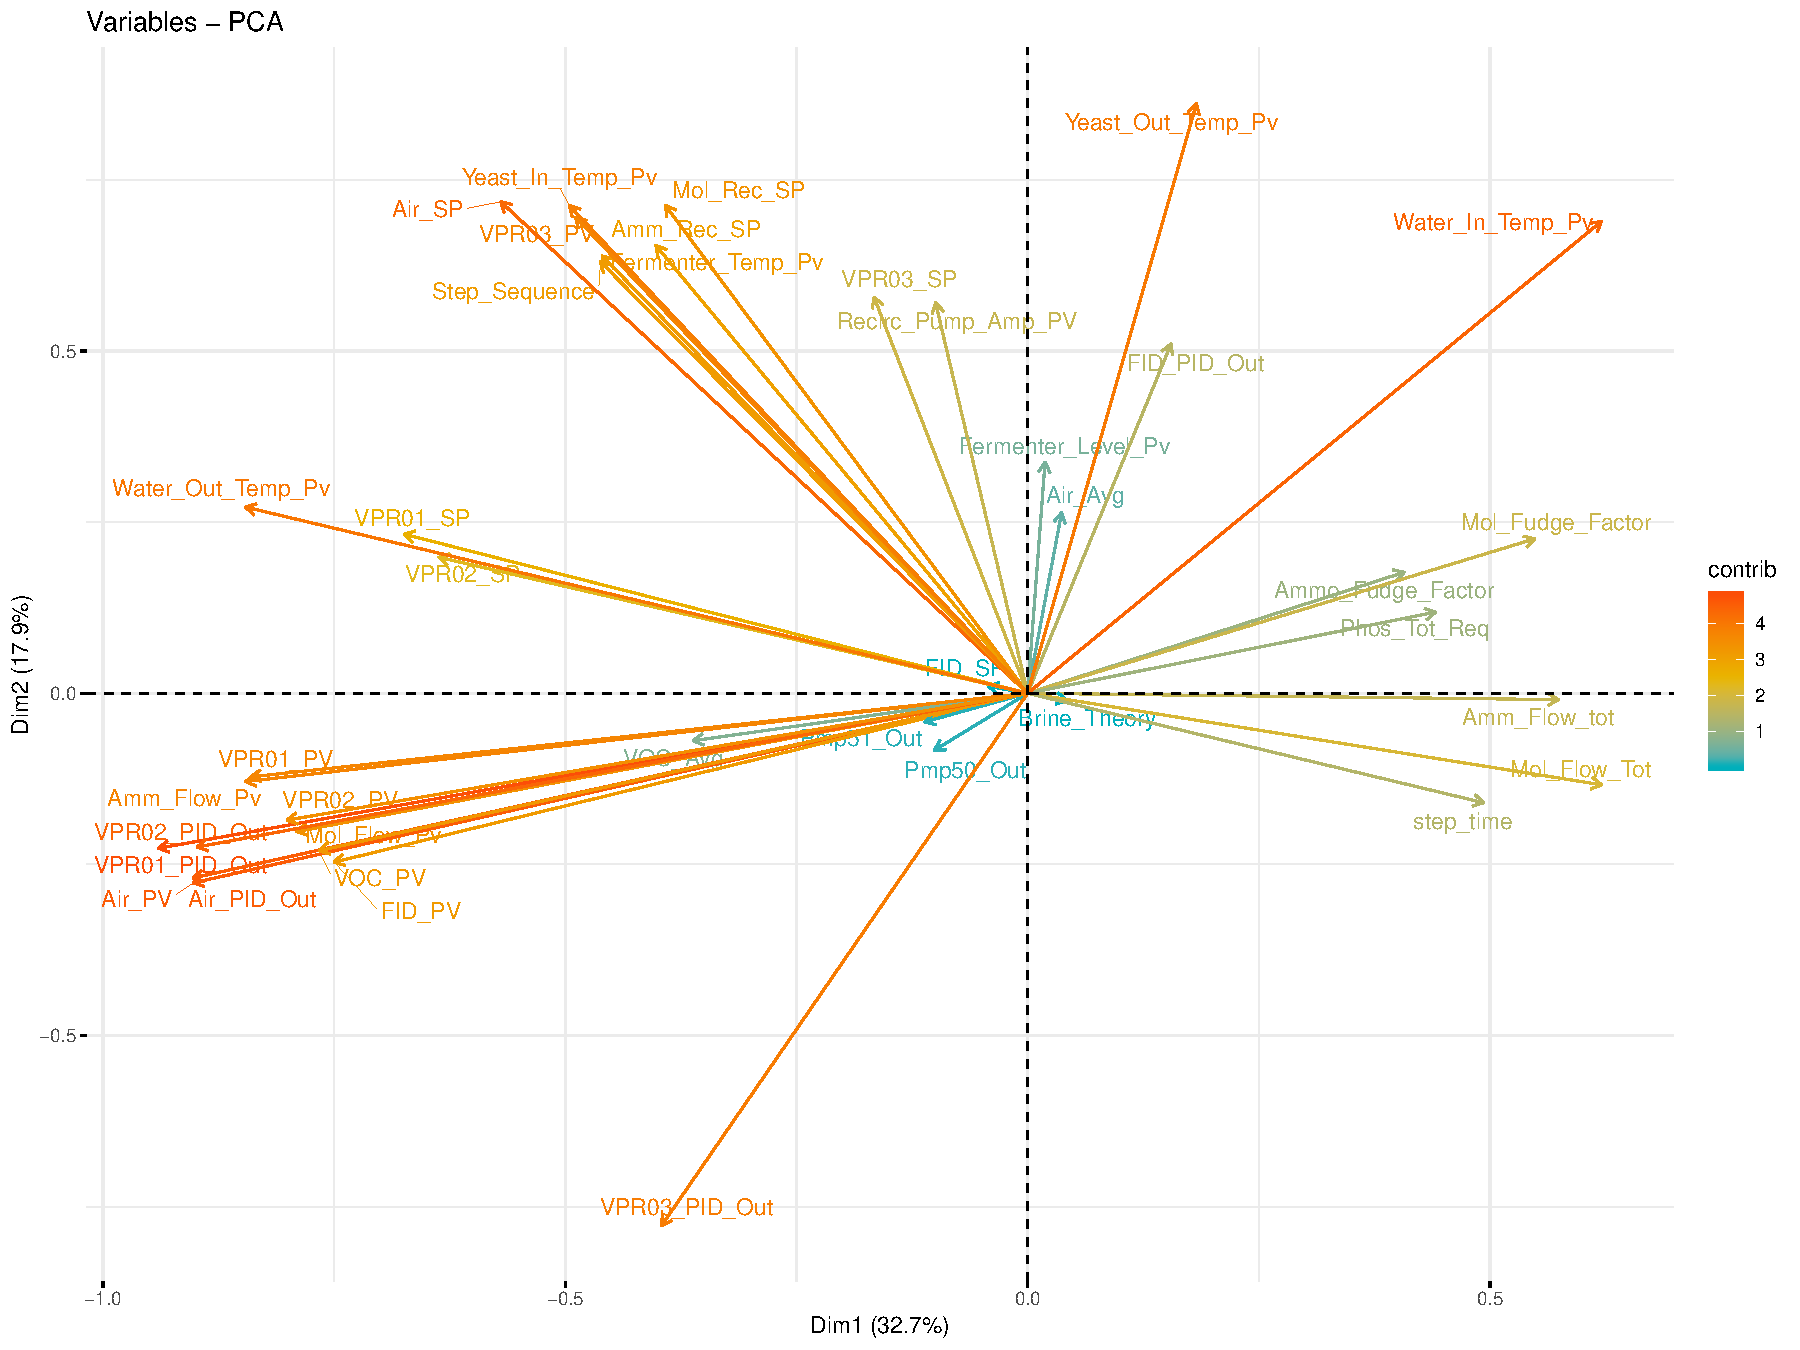
\includegraphics[width=\textwidth]{plots/f5_graph_of_variables.pdf}
        \caption{F5 Variables}
        \label{fig:f5_variables}
    \end{subfigure}%
    \begin{subfigure}{0.3\textwidth}
        \begin{center}
        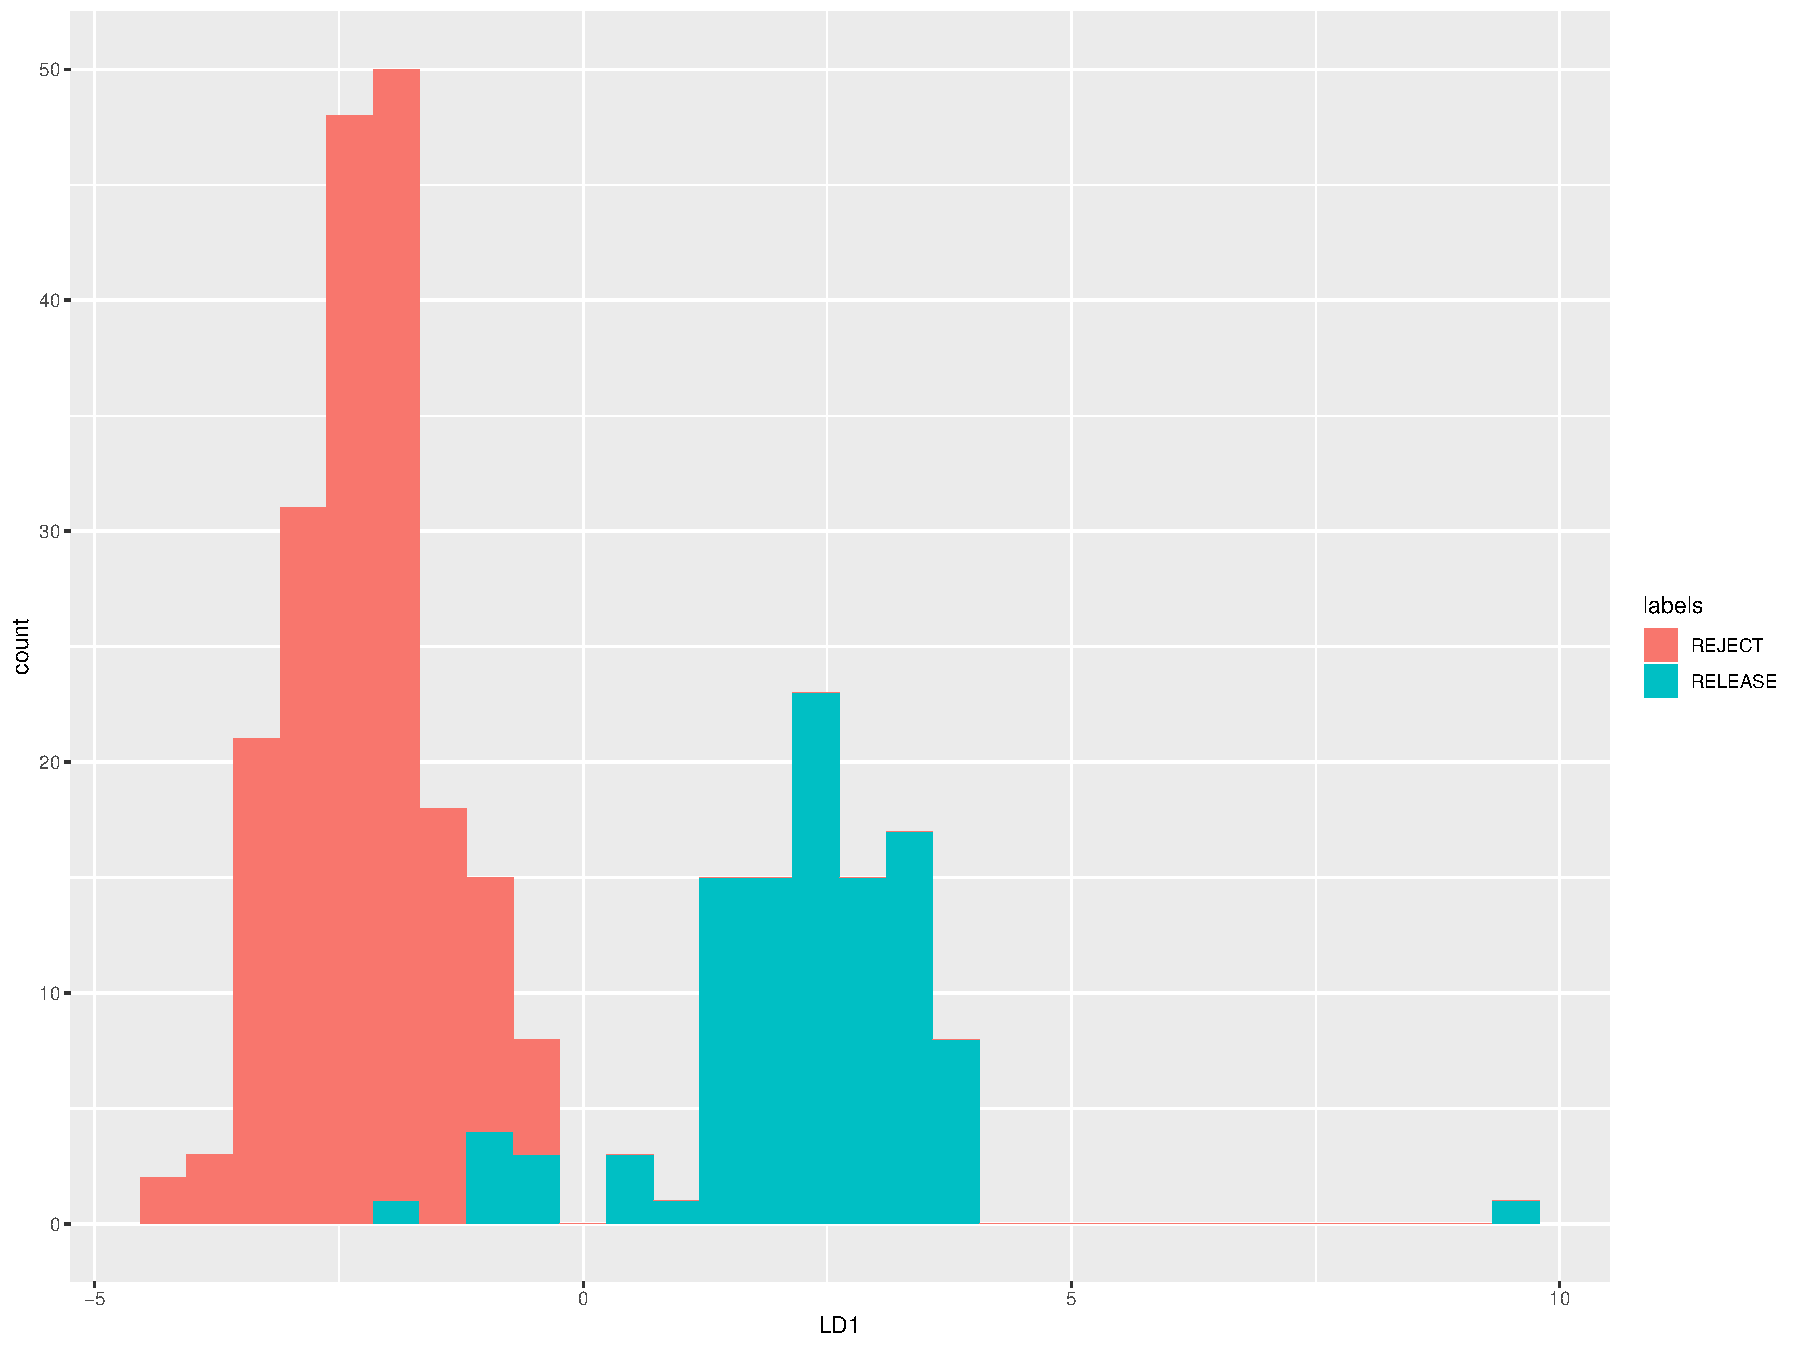
\includegraphics[width=\textwidth]{plots/f5_LD1.pdf}
        \end{center}
        \caption{F5 LD1 distribution across classes}
        \label{fig:f5_LD1}
    \end{subfigure}
    \caption{F5 component analysis}
\end{figure}

The results of LDA are displayed on Figure \ref{fig:f5_LD1}. Even though the Figure shows evidence of strong difference between ``rejected'' and ``released'', it is not reliable since the sample size are one of each class. Therefore the difference between those to production batches could be anything from environment to random chance. More than in any other production step described above, F5 required significant additional data collection to make any substantial conclusions on the process performance and stability.



% Conclusions section
\section{Conclusions}
\label{sec:conclusions}
During exploration and preparation of the given datasets the following was noticed:

\paragraph{Overall quality was acceptable} There were some N/A variables with null values or missing measurements. The variables nature (data types) vary: process duration measures of step times, constant values of temperature, air and other conditions, boolean values, etc. However, the structure of variables is not homogeneous. Mainly variables represent a specified volume or mass of ingredients from manufacturing formulas, however, the data also consist of process condition measurements, such as an air or water temperatures.
    
\paragraph{Quantities} Provided \emph{sample data} with labels/status information (eg. the quantities of products that were released and rejected) \emph{is not sufficient enough for research}. 
    
\paragraph{Manual data} Furthermore, information about \emph{seed/batch number and statuses were matched manually} and therefore significant \emph{a probability of error} may exist – not all observations may have correct references to the yeast production \emph{cycle start and end times}.
    
\paragraph{Timestamps} In some cases, Date and Time data integrity is loosely presented and the assurance that the data is correctly merged is not consistent.
    
\paragraph{Classification} Even though the prediction of the status within given parameters was not very reliable, it was still possible. In the future, with improved input data (better matching and more class samples), the prediction precision could be increased.

\paragraph{Analysis conclusions} From the data analysis the following can be concluded:
\begin{itemize}
    \item The dataset is currently too small and unbalanced to produce statistically significant and reliable results. Moreover, the dataset is not sufficient yet to build reliable machine learning models.
    \item The variance between the process data of ``rejected'' and ``released'' batches appears to be significant in process step F2 and substantiates further research, whether these difference can influence the mutations and the quality of the yeast.
    \item In steps F4 and F5 the data is inconclusive and at current state is not able to provide any interesting insight. We recommend to collect more data, see Recommendations section of this paper.
\end{itemize}

% Recommendations section
\section{Recommendations}
Having completed the initial analysis of the yeast production process we have the following recommendations for further process improvements and better analytical insight:

\begin{itemize}
\item Digitize and automate if possible the current manual data collection on the production batches that is at present time in a form of scanned PDF files. The current system is error prone and does not lend itself easily for analytics.
\item Consider automatic loading of process data that is currently in CSV files into a time series database. That will provide for long term data storage and ease the preparatory steps for any future analytics on the fermentation process.
\end{itemize}

\subsection{Data Collection}
\paragraph{Labelling of parametric data with quality control information.}
Currently the classification and labelling of production batches is done manually, by guessing the batch production start and end times and labelling the recorded data accordingly. Therefore, the quality of labelling is a potential source of inaccuracies. The question of \emph{which measurements correspond to ‘Rejected’ and which ones correspond to ’Released’ statuses and  which measurements belongs to ‘Seed’ number 4151 and which ones to ‘Seed’ number 5292?} should be answered automatically.

\paragraph{Glossary} For further analysis and data storage create data glossary that describes all variables and terms used. This will limit possible future confusions in interpreting the data. Such glossary and metadata is an important portion of organizational data governance and data management.

Additionally, in order to analyze the parameters collected from the yeast cultivation process online (and offline) and identifying the deviations that cause quality problems, it is required to have enough historical data that allows to capture information about exact batch numbers and statuses with regards to time and production cycle. 

\paragraph{Automation of currently manual data collection.}
Recommend to automate collection of status information such as:
\begin{itemize}
    \item Production Date (MM-DD-YYYY)
    \item Strain
    \item Seed batch number
    \item Commercial batch number
    \item Lot no
    \item Status - quality control decision: Rejected, Released, Restricted release
\end{itemize}

Currently the relationship between time series data from separate production steps is merged and matched manually (eg. linking steps F2 and F4). That linkage should be automated.

\paragraph{Grouping parametric data into production batches.}
Every time\-stamped row of parametric data should be grouped into a respective production batch. As many observations belong to the one production batch (M:1) that means approx. 3 days duration for the one particular seed/batch, so after matching the data it should not have \emph{gaps or overlaps} in time period.  

Proposed new records to process parametric time series data on production batches: 
\begin{itemize}
    \item production line active / not active
    \item new batch start point / no change
    \item batch standing / running (batch serial number has to be assigned) 
\end{itemize}

\paragraph{Paperless Data Collection Consideration.}
\begin{itemize}
    \item Data provided on fermentation sheets (ie "7442ferm sheets"), contains manually measured values of the pH, spin test and other necessary variables. However they are \emph{not currently sufficient for analysis} and it is required to \emph{collect such historical data in digital and preferably automated manner}. 
    \item Making some fields ‘mandatory’ helps to submit data without missing it and therefore increase \emph{data completeness} (whether there are any gaps in the data from what was expected to be collected, and what was actually collected).
    \item Make sure that \emph{data integrity} is enforced. That is, that the data has not been changed when performing any operation on them, whether it is transfer, storage, display or during data preparation.
\end{itemize}

\subsection{Data Preparation}
To improve data preparation historical data instead of CSV files could be stored in some database tables or at least \emph{previously merged files corresponding to original time stamp and business process step}.

The main idea here is to have  precise mapping of date and time along the whole process to be able to monitor 1 batch from start to end like a holistic process work flow (for example to merge events from F1 $\,\to\,$ F2 $\,\to\,$ F4 steps vertically or horizontally, following and keeping  the full production time interval (approx. 3 days) required for producing the one yeast seed /batch.) 

Yeast separation, storage container data could be also referred to batch, seed and production dates. 

\subsection{Data Analysis}
We propose the following improvements for future data analyses:

\paragraph{Additional data collection.} Having more samples with labelled observations (Strain, Seed, Status) give higher probability to identify deviations that cause quality problem, identify which variables measurements impact quality and predict the production result /status.
\paragraph{Digitize manual data.} Having paperless recorded variables (i.e. pH) included to modelling to allow for more holistic analysis and modelling of the collected parameters. 


% Areas of further study
\section{Areas of Further Study}
Since the scope of this analysis was limited and aimed rather at proving the potential, we identified but did not cover the following potential areas of further research:

\paragraph{Include pH levels to the time series data.} Currently only automatically collected data was analyzed and modelled. In further work, also the data collected manually (or currently in PDF form but not easily readable) should be incorporated to to modelling. The working hypothesis of that research would be, that dynamics of pH level has statistically significant impact on the undesired mutations in yeast.
\paragraph{Perform more advanced feature engineering on the collected process data.} Currently the process data was treated as independent points in time series. However describing the features of each individual time series for a production batch (such as shape of the curve, rates of change, variablities, moving averages etc) could provide additional valuable insight for modelling. However, it should be noted, that such aggregation of process data will introduce micronumerocity (ie. making sample sizes even smaller). Therefore, in order to provide statistically significant results, firstly, more data collection is needed.

\appendix
% Data description table goes to annex
\begin{landscape}
\section{Data Description}
\begin{center}
\begin{longtable}{l | p{5cm} | p{1.5cm} | p{10cm}}
\label{tab:data}
No & Data Source &	Data Origin	& Description \\
\hline
1 &	F1 data, 2 csv files	& provided & \\
2 &	F2 data,  5 csv files	& provided &	49092 rows, 0-211 cycles, 44 var, Initial fermentation data \\
3 & F4 data, 7 csv files	& provided &	49092 rows, 0-213 cycles, 60 var, yeast product data \\
4 &	F5 data, 6 csv files	& provided &	49093 rows, 0-282 cycles, 52 var, Commercial yeast product data \\
5 &	F7 data, 6 csv files	& provided &	49092 rows, 0-225 cycles, 52 variables \\
6 &	F8 data, 6 csv files	& provided &	49092 rows, 0-135 cycles, 52 variables\\
7 & CSep data, 3 csv files	&provided \\	
8 &	MO data, 17 csv files	&provided \\	
9 &	Seps data, 9 csv files	&provided \\	
10&	SR data, 11 csv files	&provided \\
11&	Manual fermentation recordings,  
F2-F4 10 pdf, F5 2 pdf files&	provided&	processes manually filled in pdf. Data contains only F4 and F5 fermentations recordings  \\
12&	Brown colonies ferms, word doc
(Quality control results for few F4 and F5 batches)	&provided&	Data has attributes
\begin{itemize}
    \item Production Date (MM-DD-YYYY) -finished product date
    \item Strain (yeast strain no 7442 only)
    \item Seed - batch number
    \item Commercial – if F5
    \item Lot no - number of batches
    \item 	Status - quality control decision: Rejected, Released, Restricted release)
\end{itemize} \\
13&	Data Parameters - Excel with fermentation variable details  	&provided&Glossary, some variables description. Mainly variables represent a specified volume or mass of ingredients from yeast manufacturing formulas, also process condition measurements, such as an air or water temperatures, etc.\\

14&	Labelled Dataset - samples with statuses 
\begin{itemize}
    \item F2 samples: 1469 obs. of 45 variables
    \item F4 samples: 1252 obs. of 62 variables
    \item F5 samples: 294 obs. of 54 variables
\end{itemize}
&created& 	
Based on provided manual notes and quality control results.  
For few F2, F4 and F5 data there were manually assigned labels (statuses): \begin{itemize}
    \item REJECT
    \item RELEASE
    \item RESTRICT
\end{itemize}
\\
\hline
\end{longtable}
\end{center}
\end{landscape}

\section{Correlation plots of the parametric data}

\begin{figure}[ht]
    \centering
    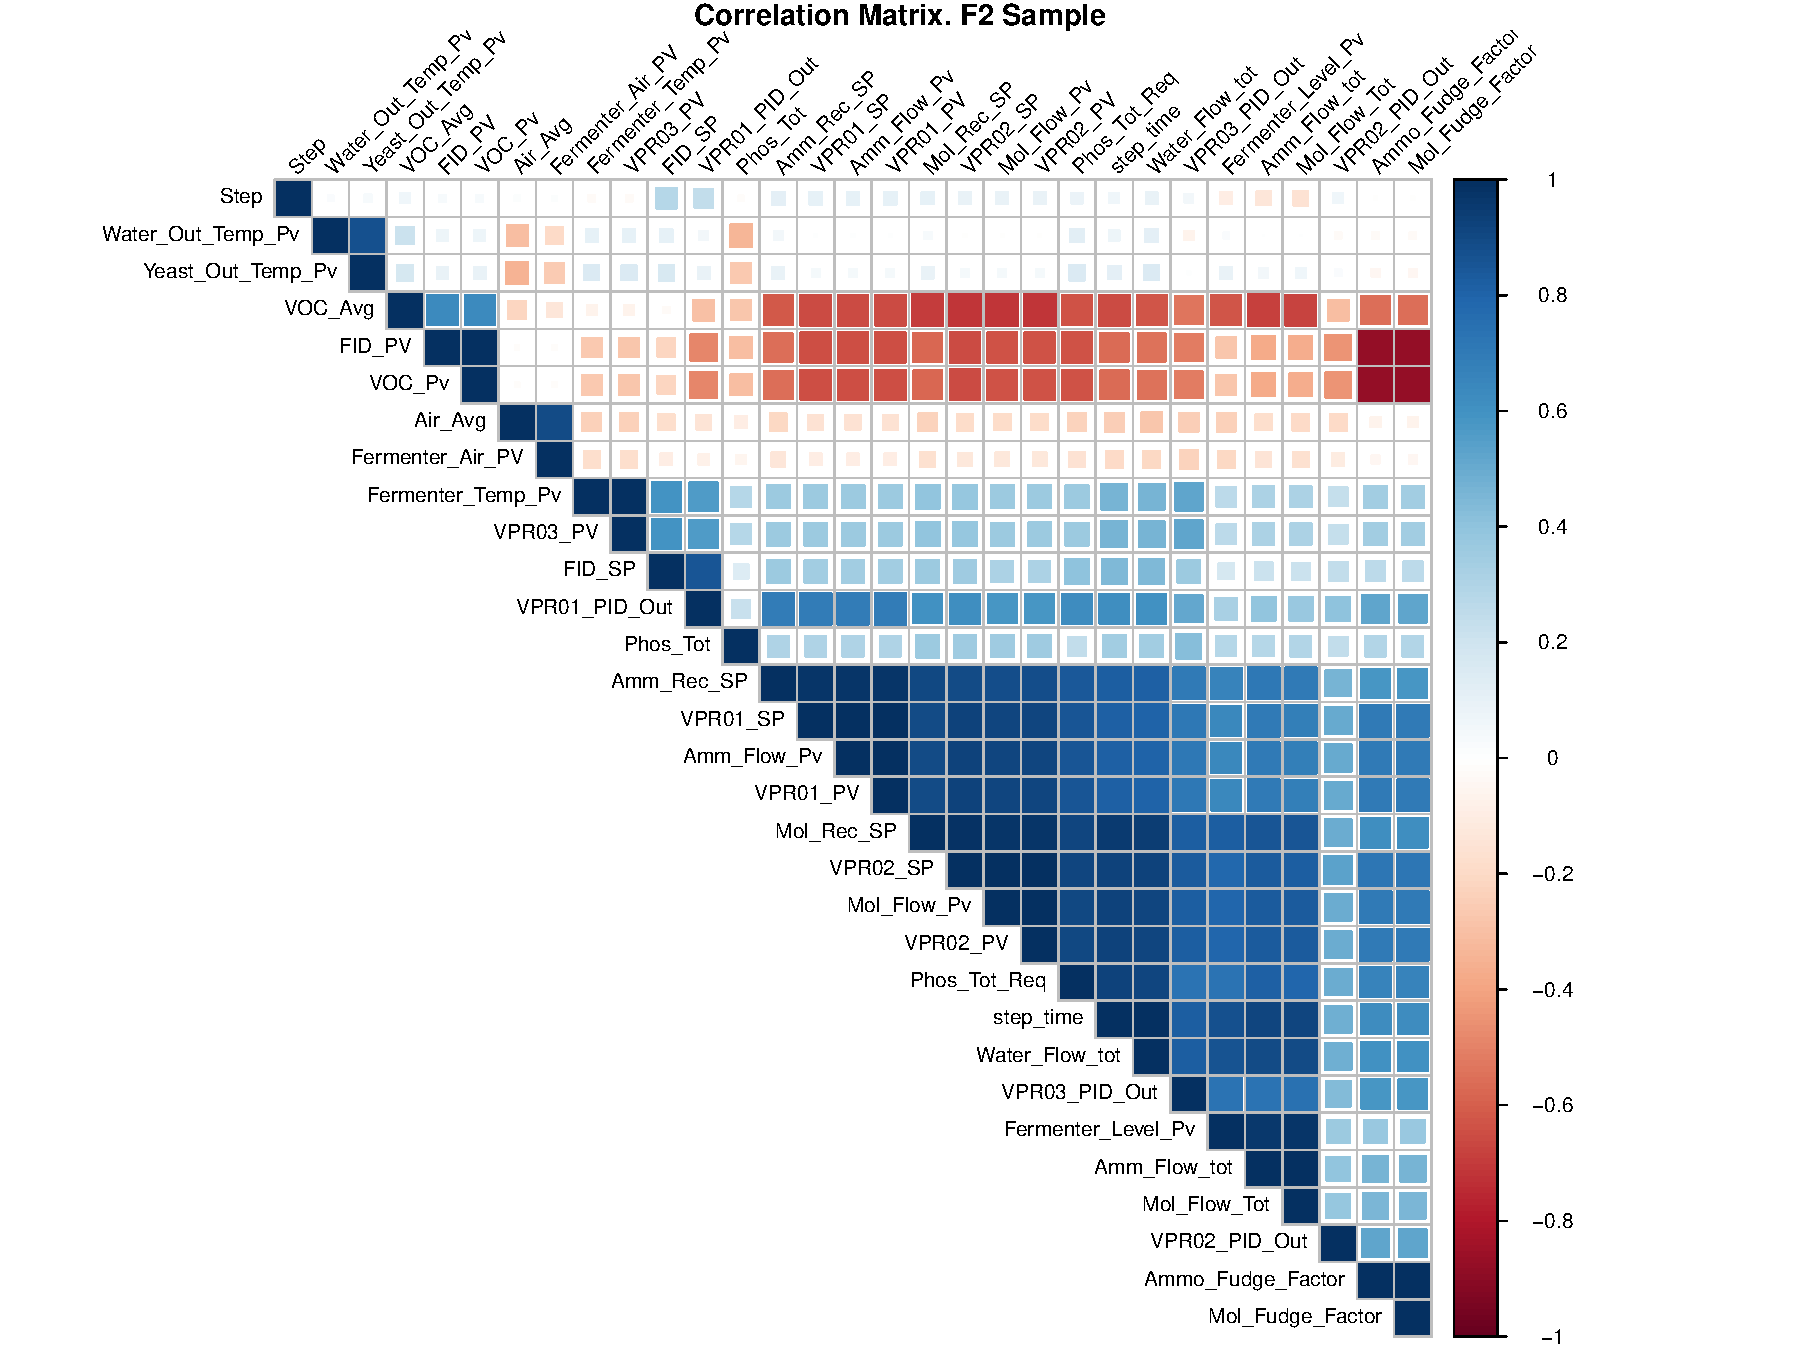
\includegraphics[width=1\textwidth]{plots/f2_correlation.pdf}
    \caption{F2 correlation matrix}
    \label{fig:f2_correlation}
\end{figure}

\begin{figure}[ht]
    \centering
    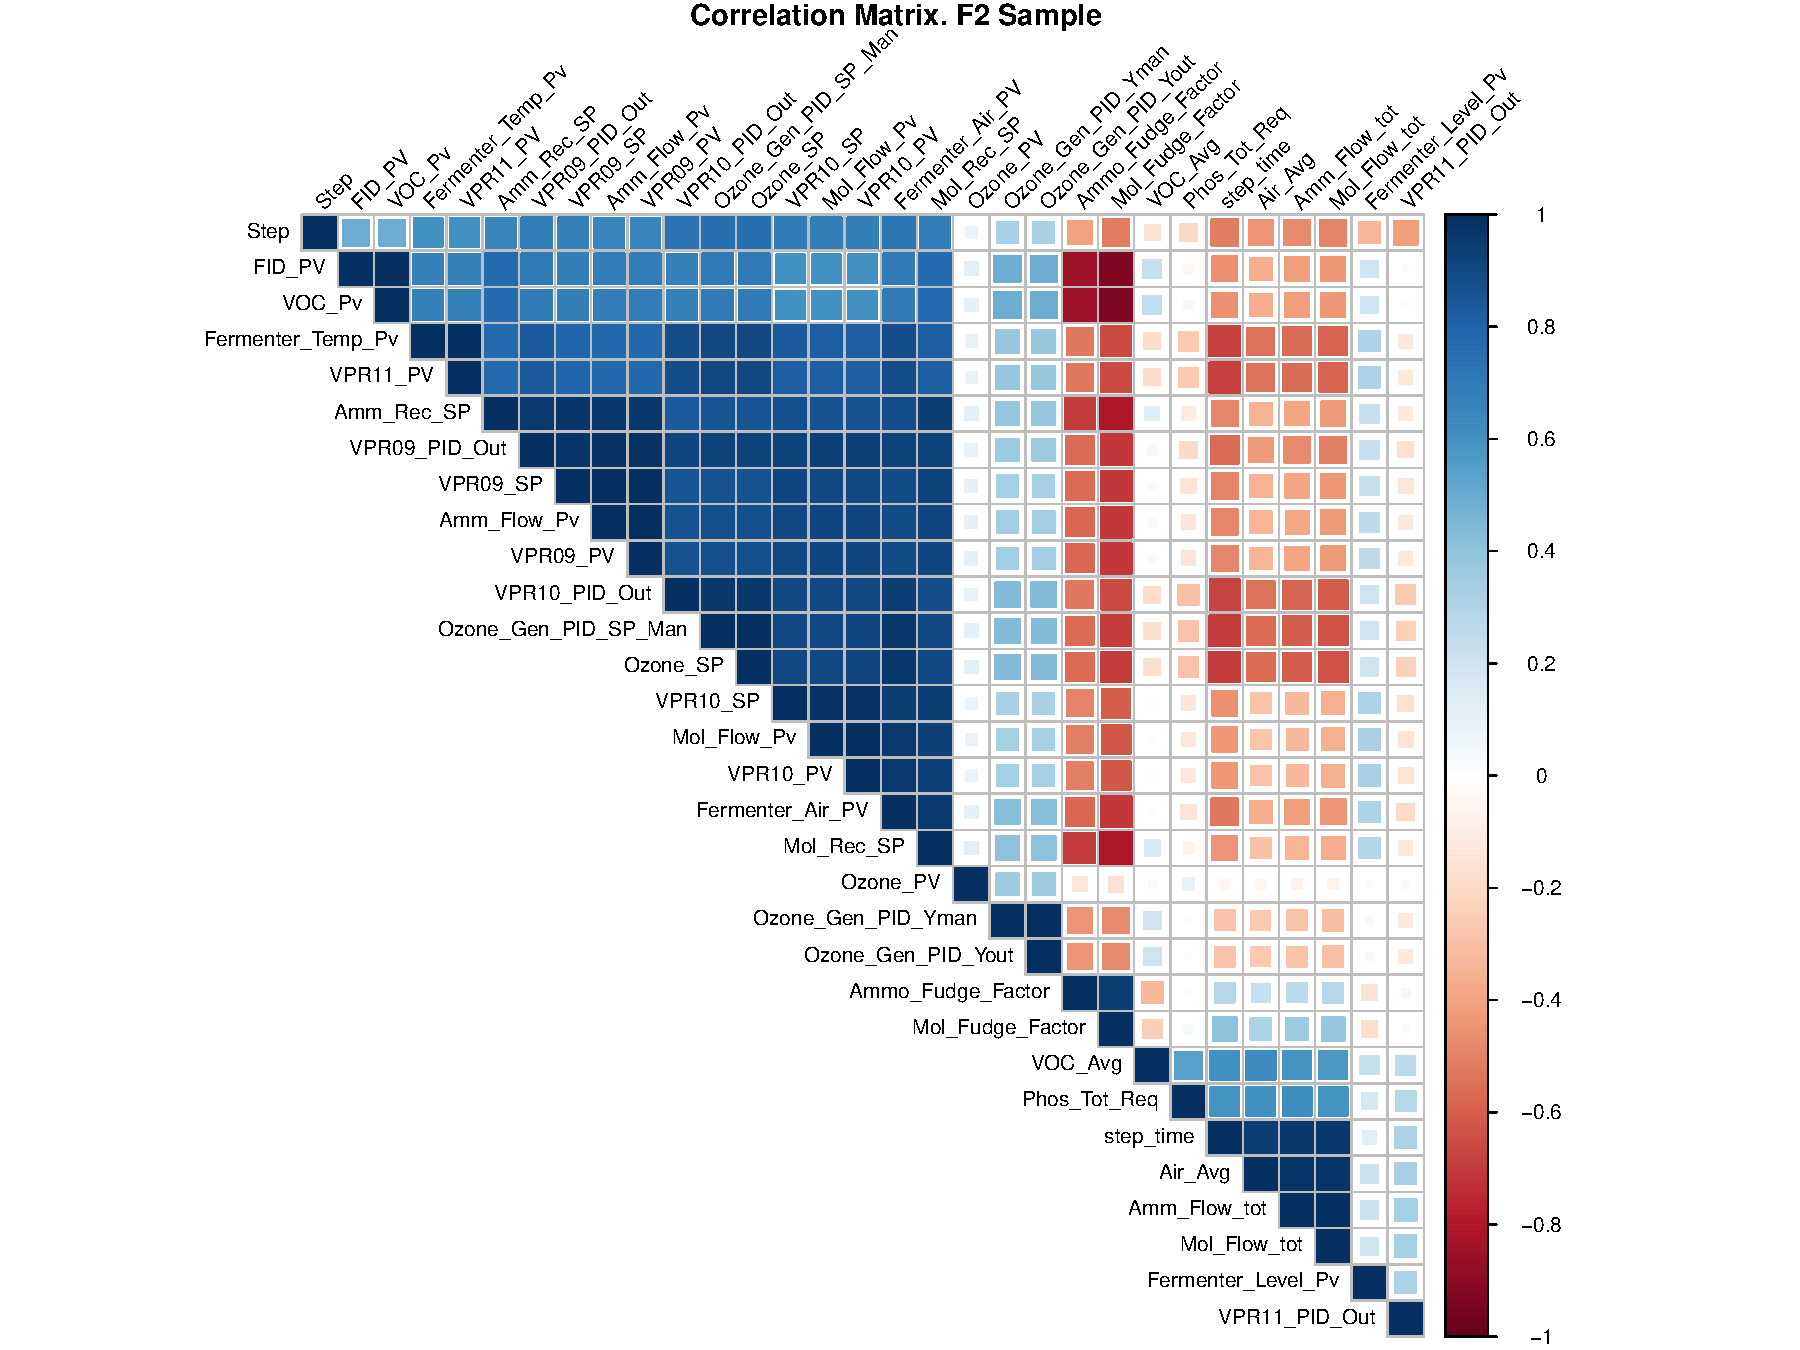
\includegraphics[width=1\textwidth]{plots/f4_correlation.pdf}
    \caption{F4 correlation matrix}
    \label{fig:f4_correlation}
\end{figure}

\begin{figure}[ht]
    \centering
    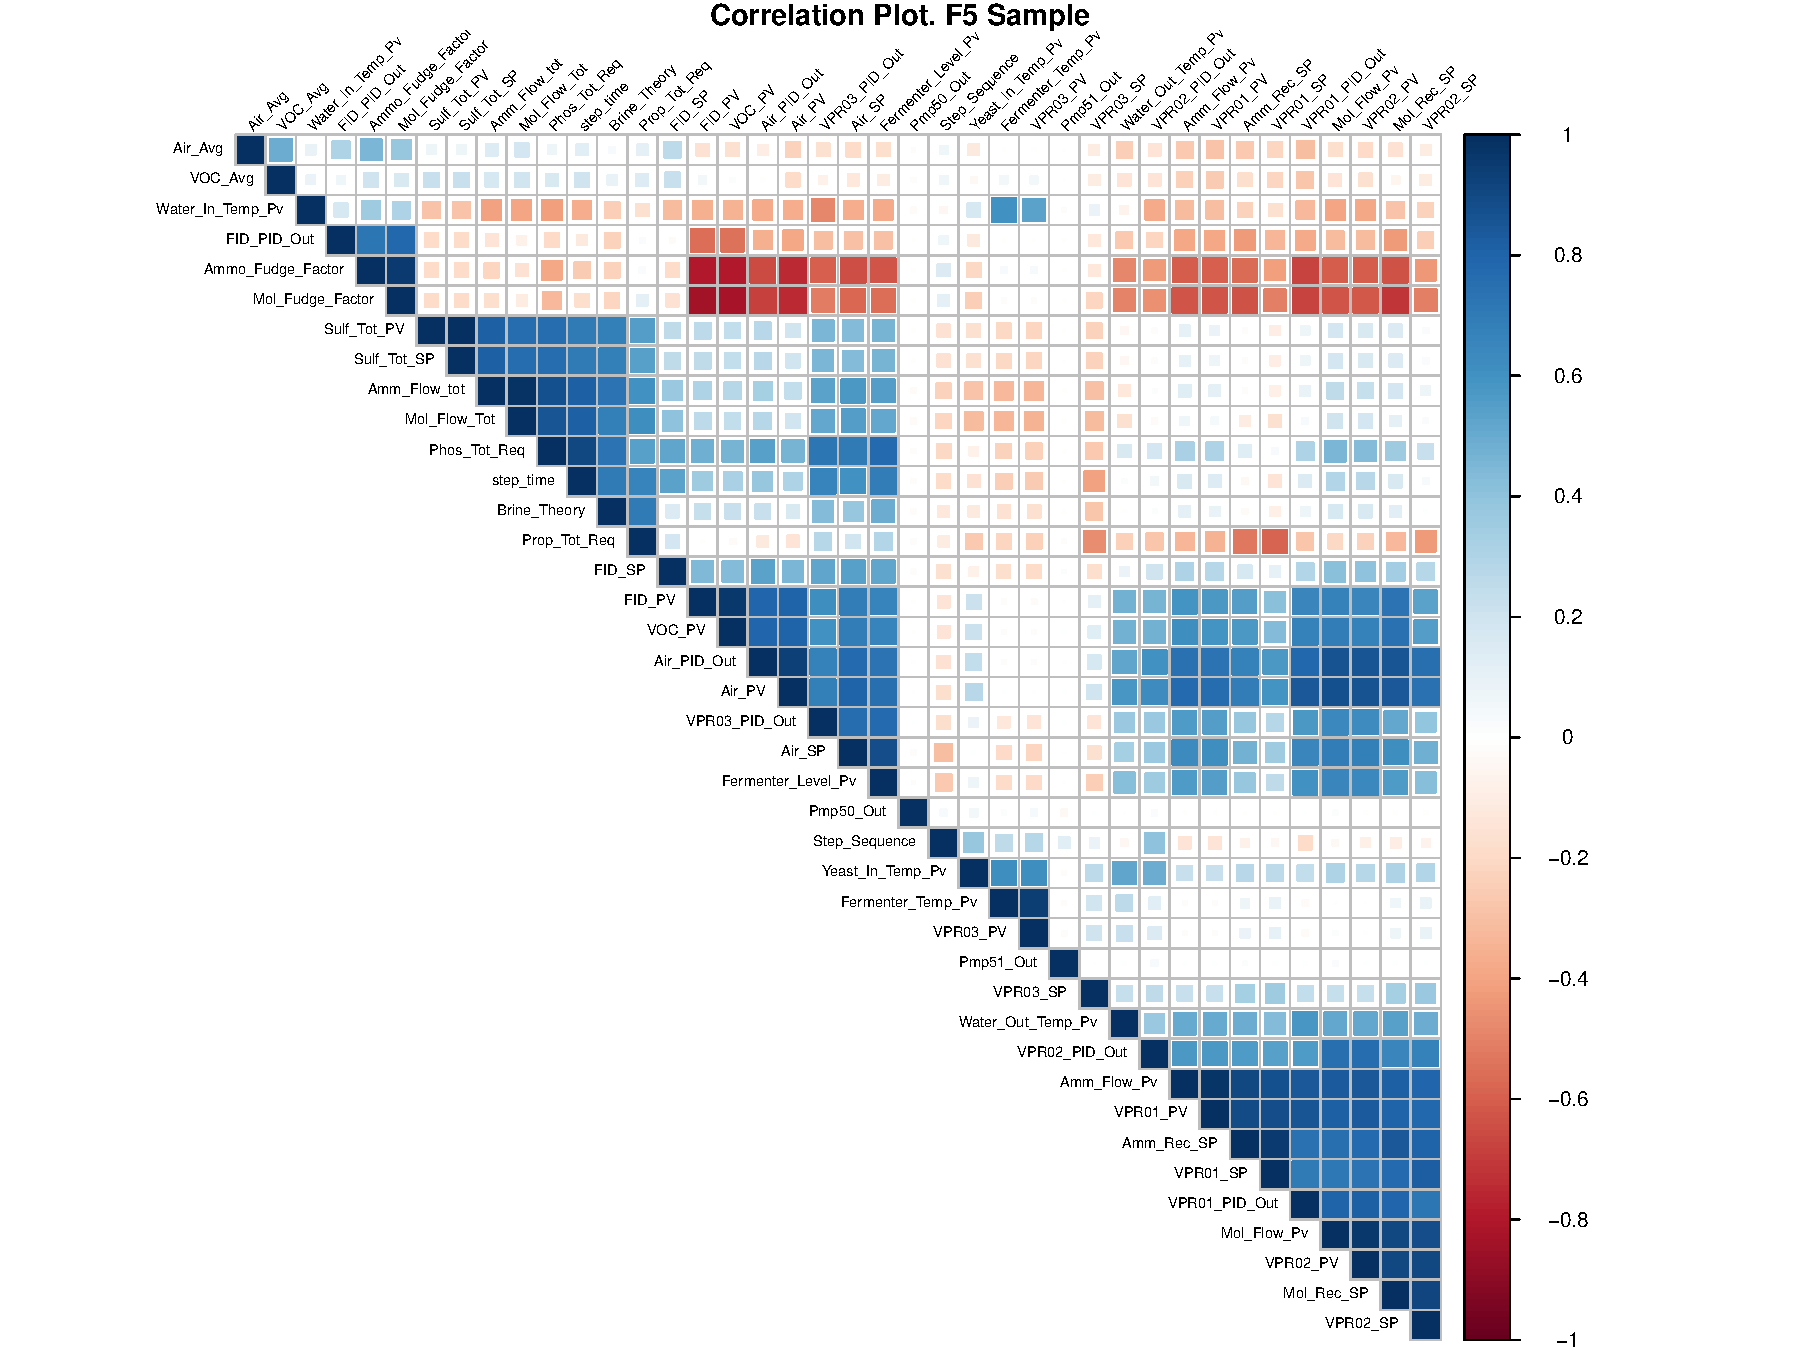
\includegraphics[width=1\textwidth]{plots/f5_sample_correlation.pdf}
    \caption{F5 correlation matrix}
    \label{fig:f5_correlation}
\end{figure}




\end{document}
